% !TeX spellcheck = hu_HU
\documentclass[12pt,a4]{article}
\usepackage{xurl}
\usepackage{graphicx}
\usepackage{wrapfig}
\usepackage{lipsum}
\usepackage{amsmath}
\usepackage{amssymb}
\usepackage[super]{nth}
\usepackage{graphicx}
\usepackage[section]{placeins}
\usepackage{mdframed}
\usepackage{hyperref}
\usepackage{caption}
\usepackage{multirow}
\usepackage{subcaption}
\usepackage{indentfirst}
\usepackage{multicol}
\usepackage{mathtools}
\usepackage[figurename=Ábra]{caption}
\hypersetup{
	colorlinks=true,
	linkcolor=black,
	filecolor=magenta,      
	urlcolor=cyan,
	bookmarks=true,
	pdfpagemode=FullScreen,
}
\usepackage{array}
\newcolumntype{P}[1]{>{\centering\arraybackslash}p{#1}}
\newcolumntype{M}[1]{>{\centering\arraybackslash}m{#1}}

\hyphenation{op-er-and op-er-ands}

\def\magyarOptions{defaults=hu-min}
\PassOptionsToPackage{magyar}{babel}
\usepackage[inputenc=utf8]{uni8}

\begin{document}	
	
	\renewcommand*\contentsname{Tartalomjegyzék}	
	
	\begin{titlepage}
		\begin{figure}
			\centering
			\begin{minipage}{.5\textwidth}
				\centering
				
\includegraphics[width=.9\linewidth]{oelogo}
			\end{minipage}%
			\begin{minipage}{.5\textwidth}
				\centering
				
\includegraphics[width=.3\linewidth]{oe}
			\end{minipage}
		\end{figure}
		\vspace{0.5cm}			
		\begin{center}			
			\Large
			Óbudai Egyetem\\
			Neumann János Informatikai Kar\\
			
			\vspace*{0.5cm}
			
			\Huge
			\textbf{3D-s arckép rekonstrukciója egy 2D-s képből mesterséges intelligencia segítségével}
			\par\noindent\rule{\textwidth}{0.4pt}
			
			\vspace{0.5cm}
			\normalsize
			Reconstructing 3D face picture from single 2D picture supported by artificial intelligence
			
			\vspace{0.2cm}
			\large
			\today
			
			\vspace{1cm}
			
			Témavezető:\\
			\textbf{Vámossy Zoltán}\\
			Egyetemi docens
			
			\vspace{1cm}
			
			Készítette:\\
			\textbf{Gaál Bernát Ruben - HBGCXK\\
			Hua Nam Anh - DQ4LFK}					
		\end{center}
	\end{titlepage}
	\renewcommand*\contentsname{Tartalomjegyzék}
	\tableofcontents
	\newpage
	\par\noindent\rule{\textwidth}{0.4pt}
	\section*{Absztrakt}
	 \emph{
		A közelmúltban a mélytanuláson alapuló 3D arcrekonstrukciós módszerek
		ígéretes eredményeket mutattak mind minőség, mind hatékonyság tekintetében. A neurális hálózatok tanítása azonban jellemzően nagy mennyiségű
		adatot igényel, ami magával vonza a megfelelő erőforrásokat.
		A felsoroltak hiányában mi az alábbi megoldást javasoljuk. Egy gyengén
		felügyelt tanítású hálózatot amit, lehetséges ”in-the-wild” képekkel betanítani.
		Ennek megvalósításához kettő már kész kutatás anyagát vettük igénybe. Az
		első, \cite{deca}DECA képes kezelni az arc kisebb részleteit, arckifejezéseit. A
		másik, a \cite{focus}FOCUS bemutatott egy korszerű megközelítést az arckép rekonstrukciójára okklúziók mellet, mint például szemüveg,sapka stb. Ezek a kutatások nem csak korszerűek, de a NOW challenge benchmark-ja alapján bizonyitottan jól teljesítenek. Ezeket ötvözve egy robosztus, illetve realisztikus
		arcképek generálására alkalmas módszert mutatunk be ebben a tanulmányban.
		A rekonstrukció mellet implementáltunk egy arckép analízálására alkalmas módszert, amely képes eldönteni az arcképen lévő személy érzelmi
		állapotát és korát. Ezek köré egy felhasználó barát microservice alapú web
		applikációt biztosítunk, melynek szolgáltatásai felhőn üzelmelnek.
		}
	 \par\noindent\rule{\textwidth}{0.4pt}
	 
\section{Bevezetés}
	  
	   Az elmúlt évek során, egyre több figyelmet kaptak a digitális
	 képfeldolgozáson alapuló technológiák az informatikában. Mint ahogy \cite{survey} is megvan említve az arcfelismerő technológiák széles
	 körben elterjedtek napjainkban, beleértve a biztonságot, animációt és egészségügyet. Illetve, ezen szakmai területen mostanság felkapott,
	 hogy 3D-s adatok implementálásával megkerüljék a 2D arckép által megszabott határokat, mivel a 2D-s kép képtelen az emberi arc geometriájának eltárolására.
	 A 3D arcfelismerés sokkal pontosabb adatokat ad vissza, például pózban és megvilágításban, amelyek hátulütői a 2D-nek. Azonban ennek is vannak hátrányai, mint például, hogy sokkal nagyobb komplexitású képfeldolgozást igényel, ezáltal szűkítve a lehetőségeket.
  
Az arcokat többféleképpen is lehet rögzíteni, például Stereo-vision rendszerekkel, amelyek két kamerát használnak. Ezek a kamerák ugyan arról az objektumról készítenek párhuzamosan képeket, majd ezeket összehasonlítva visszaadják a képen lévő egy pontnak a mélységét.  

Egy másik módszer a 3D lézerszkenner (pl. NextEngine, Cyberware), amelyet elsősorban ipari célokra fejlesztettek. Ipari termékek vizsgálatával szemben, az emberi arc feltérképezéséhez több feltételt kell figyelembe venni. Mivel az emberi arc nem lehet teljesen mozdulatlan, fontos, hogy a szkenner által készített felvétel időintervalluma csekély legyen.
Röviden, a lézerszkenner fényhullámokat szór az objektumra, s ezek annak felszínéről visszaverődnek a szenzorra. A szenzor ezután kiszámítja az objektum felszínének távolságát az alapján, hogy mennyi idő alatt tette meg a teljes utat a hullám. Ezt a folyamatot $"Time\enspace of\enspace flight"$-nak szokás nevezni. 
  
	 A következő technológia a 3D-s adatok rögzítésére az RGB-D kamerák (pl. Kinect) használata. Ezek olyan RGB kamerák, amelyek rendelkeznek infravörös szenzorral, mely mélységi adatokat biztosít, ezáltal egy RGB képet ad vissza, amiben minden pixelhez tartozik egy mélységi érték.
  
	 Bár, ezek a módszerek mind megfelelnek 3D-s adatok gyűjtésére, az első két megvalósítás hátránya, hogy előre megszabott feltételeknek megfelelő környezetet és drága felszereléseket igényel egy jó minőségű arc szkenneléshez. Ellenben, az RGB-D kamerák olcsóbbak és könnyebben használhatóak de a minőség korlátozott.
  
	 A fent említett megközelítések általában költséges optimalizálási folyamatot igényelnek a jó minőségű 3D-s arc visszanyerése érdekében. Két évtized telt el Vetter és Blanz úttörő munkája óta \cite{blanzvetter}, amely először mutatta be hogyan lehet egyetlen képből rekonstruálni az arc 3D-s geometriáját. Azóta a 3D arcrekonstrukciós módszerek rohamosan fejlődtek, de a korábbi modellek csak az arc durva alakját tudták rekonstruktuálni és képtelenek voltak kinyerni az arckifejezéstől függő geometriai részleteket, mint például a ráncokat, amik fontosak a realisztikusság szempontjából.
	 
    Később jöttek újabb modellek, melyek képesek voltak kiragadni a fent említett geometriai részleteket, azonban hátrányuk, hogy egy nagy volumenű,
 jó minőségű tanító adathalmazt követelnek. Illetve, egy másik hátrányuk, hogy inkonzisztens módon teljesítettek az okklúziókkal szemben. Az okklúziók mindenütt jelen vannak, és eleve nehezen kezelhetőek az alakjuk, megjelenésük és a pozíciójuk sokfélesége miatt. Ezáltal okozott probléma az, hogy az arcmodell alkalmazkodik az eltakart arcrégióhoz, és ennek eredményeként a rekonstruált arc torz lesz. Ezért fontos nyitott kérdés marad annak eldöntése, hogy mely pixelek illeszkedjenek és melyek ne illeszkedjenek az arcra egy 3D arc rekonstrukciója során okklúziók jelenlétében. A közelmúltban számos olyan módszert javasoltak, amelyek gyengén felügyelt tanítású konvolúciós neurális hálózatokat(CNN) használnak a hatékony, robosztus és a fent említett kihívásokat leküzdő arcrekonstrukció eléréséhez.
	 
    Tehát, a jelenlegi monokuláris 3D arcrekonstrukciós módszerek képesek finom geometriai részleteket visszaadni, azonban számos megkötéssel
küzdenek. Egyes módszerek olyan arcokat generálnak, amelyeket nem lehet valósághűen animálni, mivel nem modellezik, hogy hogyan változnak a ráncok az arckifejezésekkel. Más módszerek kiváló minőségű szkennelt arcokat használnak tanításhoz, és nem jól általánosíthatóak a természetes körülményekben készült képekre. A Yao Feng et. al. által bemutatott DECA model a legelső olyan megközelítés \cite{deca}, amely regresszálja a 3D arcformát és az animálható részleteket, amelyek egy személyre jellemzőek, de az arckifejezéssel változnak, ezáltal képesek az arc valósághű animálására.
	 
Az okklúziókkal szemben a legtöbb megközelítés a 3D arc illesztéséhez inverz renderelést alkalmaz egy adott eltakaró szegmentálásához. Ennek hátránya, hogy egy okklúzió szegmentációs modellhez nagy mennyiségű annotált adatra van szükség. Chunlu Li et. al \cite{focus} ezzel ellentétben egy olyan modellalapú megközelítést mutat be a 3D arc rekonstrukciójához, amely rendkívül robosztus az okklúziókkal szemben, de nem igényel semmilyen okklúziós annotációt a tanításhoz.
	 
Ebben a tanulmányban az a célunk, hogy egy olyan animálható 3D arcrekonstrukciós modellt készítsünk gyengén felügyelt tanulással, amely robosztus az okklúzió ellen, a fent említett DECA és FOCUS modellek segítségével. Ezt kiegészítve, bemutatunk egy arcképet elemző megoldást, mely visszaadja a célszemély érzelmi állapotát, illetve életkorát. Eszrevettük a munkánk elkészítése során, hogy a meglévő megoldásokat nehéz egy átlagos személynek kipróbálnia technikai tudás hiányában, így a fenti két szolgáltatás köré egy webapplikációt készítünk, amit felhőn üzelmeltetünk.\\
	 
Összefoglalva, ez a dokumentum az alábbi öt szempontot fogalmazza meg:
\begin{itemize}
	 \item Bemutatunk egy CNN-alapú, egyetlen képen alapuló arcrekonstrukciós módszert, amely kihasználja a hibrid szintű képinformációt a gyengén felügyelt tanuláshoz.
	 \item Konzisztens műkődést biztosít különböző okklúzók mellet.
	 \item Az arckifejezésektől függő geometria adatok azonosításával egy animálható realisztikus 3D arcrekonstrukciót hozunk létre.
	 \item Arc elemzésére alkalmas megoldás.
	 \item Webapplikáció elkészítése és a szolgáltatások megfelelő mükődése a felhőn
\end{itemize}

 
\section{Kapcsolódó kutatások}
 	
    Ahogy láthatjuk, különböző munkák megkísérelték a fellépő komplex kihívásokat legyőzni, minél kreatívabb megközelítéssekkel. Ezekről tovább Vetter és Blanz \cite{blanzvetter} munkájában és további dokumentumokban lehet olvasni. Ebben a fejezetben megvizsgáljuk a Yao Feng et. al. \cite{deca} valamint Chunlu Li et. al \cite{focus} által bemutatott megközelítéseket és megnézzük, hogy miért is fontosak a mi munkánk szempontjából.
 	
 	\subsection{DECA}
 	
    Yao Feng et. al.\cite{deca} az egyetlen, ”in-the-wild” 2D-s képből rekonstruált animálható 3D arcmodell készítése érdekében fejlesztették ki a DECA (Detailed Expression Capture And Animation) modelljét. Egy ”in-the-wild” képekkel tanított animálható elmozdulási modellt javasolnak, amely a kifejezési paraméterek változtatásával képes hiteles geometria részletek előállítására. Az előbbi cél elérése érdekében egy újszerű részletkonzisztencia költségfüggvényt mutatnak be a statikus és az arckifejezésekre dinamikusan változó geometriai adatok szétválasztására. Ammennyiben a tanítás során két kép érkezik különböző arckifejezésekkel, megfigyelhető, hogy a 3D arcformájuk és a személyspecifikus részleteik megegyeznek. Ezt a megfigyelést használják ki a részletkódok felcserélésével az azonos személyről készült különböző képek között, és kikényszerítik, hogy az újonnan renderelt eredmények úgy nézzenek ki, mint az eredeti, bemenetként átadott képek. A geometria részletek rekonstrukciója robosztus a jellemző okklúziókra, a pózok nagyfokú változására és a megvilágítási variációkra.
 	
 	A továbbiakban megvizsgáljuk a DECA modell működési elvét, architektúráját.
 	
 	\begin{figure}[h]	
 		\centering
 		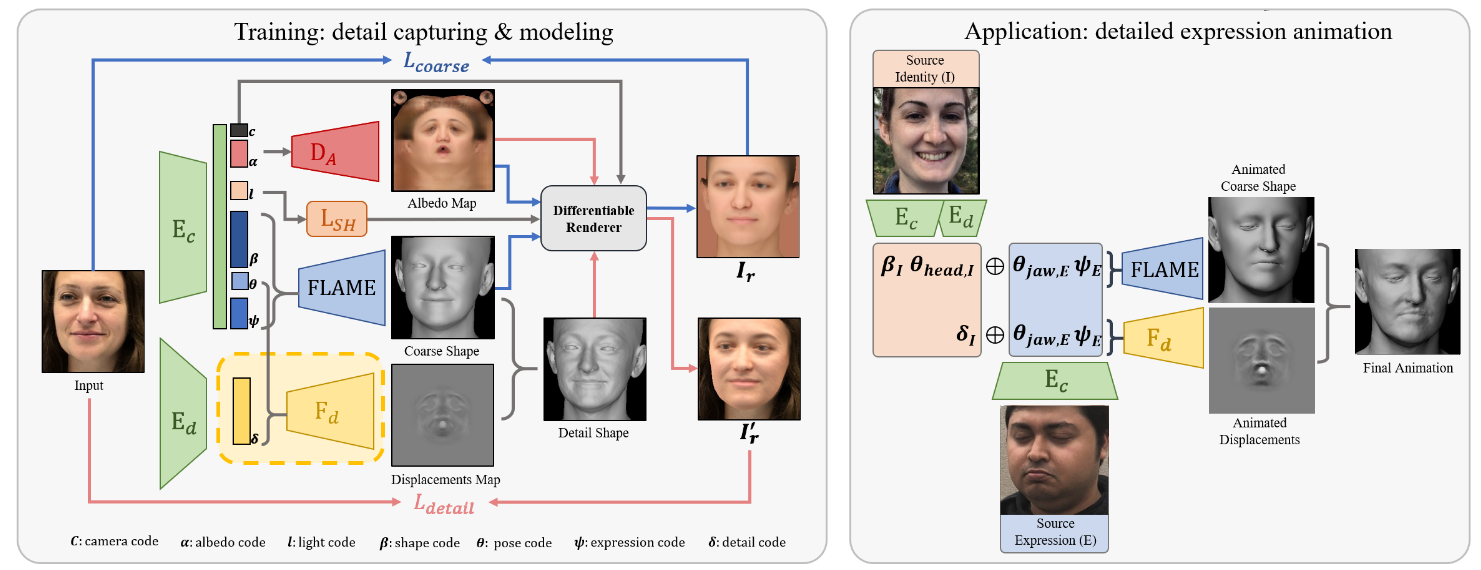
\includegraphics[width=1\linewidth]{deca}
 		\caption{ DECA tanítás és animáció.
 			Forrás:\cite{deca}}
        \label{fig:deca}
 	\end{figure}
 	
	 \subsubsection{Kódoló}
	 Első lépésként egy durva rekonstrukciót (a FLAME modelltérben \cite{flame}) tanítanak be $analysis$-$by$-$synthesis$ módon: egy bemenetként átadott \textit{I} 2D-s képből látens kódot készítenek, ezt dekódolják annak érdekében, hogy egy $I_{r}$ 2D-s képet hozzanak létre, valamint minimalizálják a szintetizált és a bemeneti kép közötti különbséget.
	 Az ábrán \ref{fig:deca} látható módon, egy $E_{c}$ kódolót tanítanak be, amely egy ResNet50 \cite{liwen} hálózatból, és egy azt követő teljesen összekapcsolt rétegből áll, egy alacsony dimenziós látens kód regressziója céljából. Ez a látens kód tartalmazza a $\omega$ (identitás), $\psi$ (kifejezés), $\theta$ (póz) FLAME \cite{flame} paramétereket(azaz reprezentálja a durva geometriát), az albedó együtthatókat $\alpha$, a kamera $c$ és a megvilágítási $I$ paramétereket.\\
	 
 \subsubsection{Dekódoló}
 	 
 	A dekódoló hálózat egy részletes $UV$ elmozdulási térképpel $D$ egészíti
 	ki a durva $FLAME$ geometriát. A durva rekonstrukcióhoz hasonlóan
 	egy $E_{d}$ kódolót tanítanak be (amelynek architektúrája megegyezik az $E_{c}$
 	felépítésével), hogy az $I$ 2D-s képből egy 128 dimenziós látens kódot $\delta$
 	készítsen, amely az alanyspecifikus részleteket reprezentálja. A látens kódot $\delta$
 	ezután a $FLAME$ $\psi$ kifejezés és állkapocs póz $\theta_{jaw}$ paramétereivel kapcsolják
 	össze, majd $F_{d}$ az imént említett paraméterekből előállítja $D$-t. $F_{d}$ a látens kódot $\delta$ felhasználva szabályozza a statikus személyspecifikus részleteket. Kihasználja a durva rekonstrukcióból kapott arckifejezés $\psi$, és az állkapocs $\theta_{jaw}$ paramétereket a dinamikus, kifejezésektől függő ráncok részleteinek rögzítése érdekében. A rendereléshez $D$-t normáltérképpé alakítják.
 	 
 \subsubsection{Részletkonzisztencia veszteség}
	 
	 \begin{figure}[h]	
	 	\centering
	 	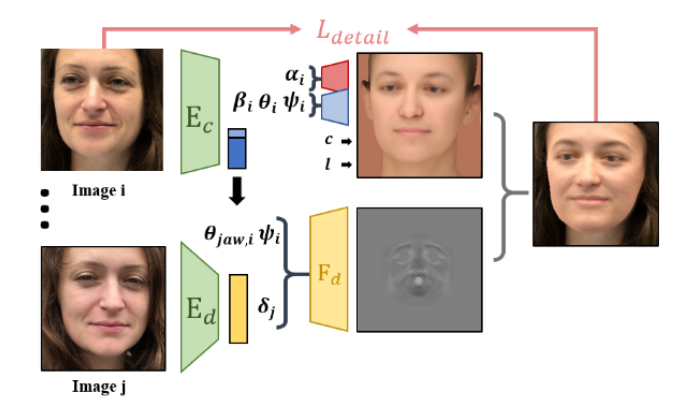
\includegraphics[width=1\linewidth]{ldetail}
	 	\caption{Részletkonzisztencia veszteség \\
	 		Forrás:\cite{deca}}
        \label{fig:ldetail}
	 \end{figure}
 
 	Yao Feng et al. az identitás-függő és a kifejezésektől függő részletek
 	szétválasztása érdekében egy új részletkonzisztencia veszteség függvényt
 	javasolnak. A metódus nélkül a személyspecifikus látens kód $\delta$ rögzíti az iden-
 	titástól és a kifejezésektől függő részleteket. Ebből kifolyólag a rekonstruált
 	részletek nem repozicionálhatóak a FLAME állkapocs póz $\theta_{jaw}$ és arckifejezés $\psi$
 	paramétereinek megváltoztatásával.
 	Amennyiben adott két kép $I_{i}$ és $I_{j}$ ugyanarról az alanyról ($c_{i} = c{j}$ ), a
 	veszteséget a következőképpen határozzuk meg:

    \begin{equation*}
    L_{dc} = L_{detail}(I_{i}, R(M (\beta_{i}, \theta_{i}, \psi_{i}), A(\alpha_{i}), F_{d}(\delta_{j} , \psi_{i}, \theta_{jaw,i}), l_{i}, c_{i}))
    \end{equation*}
   
 	, ahol $\beta_{i},$ $\theta_{i},$ $\theta_{jaw,i},$ $\alpha_{i},$ és $c_{i}$ $I_{i}$ paraméterei, valamint $\delta_{j}$ $I_{j}$ részletkódja.
 	
 	\subsubsection{Tanítás}
 	
 	Ebben az alfejezetben a(z) \ref{fig:deca}. ábrán szemléltetett $DECA$ modellt
 	vizsgáljuk meg.
 	A tanítás során (bal oldali doboz) a $DECA$ minden egyes képhez
 	az arc alakjának rekonstruálásához szükséges paramétereket becsli meg az
 	alakkonzisztencia információ segítségével (a kék nyilakat követve), majd
 	a részletkonzisztenica-információ (a piros nyilakat követve) kihasználásával
 	megtanul egy kifejezésfüggő elmozdulási modellt. A sárga doboz tartalmazza
 	az elmozdulási konzisztencia-veszteséget, amelyet részletesebben a(z) \ref{fig:ldetail}. ábra
 	szemléltet.
 	A tanítás után a $DECA$ animál egy arcot (\ref{fig:deca}. ábra, jobb oldali doboz)
 	a rekonstruált forrásidentitás alakjának, fejpózának, részletkódjának
 	valamint a forráskifejezés állkapocs pózának és arckifejezési paramétereinek
 	kombinálásával, annak érdekében, hogy egy animált durva alakot és egy
 	animált elmozdulási térképet kapjon. A modell kimenete egy animált
 	részletes alakzat.
 	
 	\subsubsection{Adathalmazok}
 	
 	A $DECA$-t három nyilvánosan elérhető adathalmazon tanítják:
 	\begin{itemize}
 		\item VGGFACE2
 		\item BUPT-Balancedface
 		\item VoxCeleb2
 	\end{itemize}
 
 	A VGGFace2 több, mint 8 ezer alany képeit tartalmazza, átlagosan több,
 	mint 350 képpel alanyonként. A BUPT-Balancedface 7 ezer képet kínál
 	etnikumonként, és a VoxCeleb2 pedig 145 ezer videót tartalmaz 6 ezer
 	különböző alanyról. összességében a DECA-t 2 millió képpel tanították
 	be.
 	
 	\subsection{FOCUS}
 	
 	Chunlu Li et. al \cite{focus} megközelítése a korábbi munkákhoz képest azért
 	különleges mert, a 3D-s arcok rekonstrukcióját és a kitakarások szegmentálását
 	együttesen végzi. Ráadásul, az általuk fejlesztett pipeline csak gyenge felügyelet mellett tanul, és nincsen szüksége annotációkra a különböző típusú
 	okklúziókhoz.
 	Ezenkivül, az általuk használt arc autoencoder lehetővé teszi az arcmodell hatékonyabb illesztését. Ahhoz, hogy növelni tudják a megvilágítással és
 	más tényezőkkel szembeni robosztusságot, implementáltak egy úgynevezett
 	perceptuális költségfüggvényt, amellyel a szegmentáló hálózat képes a szemantikus jellemzők helyett csak a független pixeleken keresztül gondolkodni.
 	
 	\begin{figure}[h]	
 		\centering
 		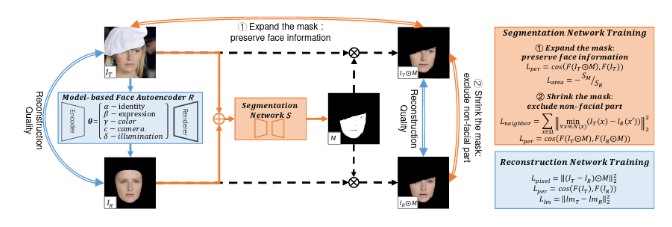
\includegraphics[width=1\linewidth]{focus}
 		\caption{Chunlu Li és tsai. által javasolt megközelítés felépítése.
 			Forrás:\cite{focus}}
        \label{fig:focus}
 	\end{figure}
 	
 	A fenti ábrán láthatjuk a $FOCUS$ hálózat felépítését.
 	Adott egy $I_{T}$ bemeneti kép, a rekonstrukciós hálózat, $R$, megbecsüli a látens
 	paramétereket és ezt követően egy olyan $I_{R}$ képet állít elő, amely csak az
 	arcot tartalmazza. Ezután az $I_{T}$ és $I_{R}$ képeket betápláljuk az $S$ szegmentáló
 	hálózatba, amely megjósolja az $M$ szegmentációs maszkot. A szaggatott
 	vonalak azt mutatják, hogy $M$-et arra használják, hogy az $I_{T}$ és $I_{R}$ képekben
 	a becsült kitakaró tényezőket kiszűrjék a képből, ezáltal összerakott kitakarás mentes képeket
 	kapnak, nevezetesen $I_{T}\bigodot M$ és $I_{R}\bigodot M$ .
 	Megfigyelhetjük, hogy Chunlu Li et. al nagy hangsúlyt fektettek bele a
 	robosztus arcrekonstrukcióra kitakarások mellet. A munkánk szempontjából
 	azért fontos, mert az arcot kitakaró tényezők mindenütt jelen vannak. Ezért is választottuk
 	a $FOCUS$-t, mert nekik sikerült egy speciális modellt implementálni, ami
 	képes kezelni a kitakarásokat anélkül, hogy szükséges lenne nagy mennyiségű
 	adatra vagy olyan erőforrásra, amihez nincs hozzáférésünk.
 	A továbbiakban részletesebben megvizsgáljuk a $FOCUS$ építőelemeit és
 	együttműködésüket.
 	
 	Ahogy, már korábban is említve volt, a $FOCUS$ célja 3D-s
 	arcrekonstrukció egyetlen képből, súlyos kitakarások esetén is. Ezen kihívást
 	jelentő probléma megoldásához egy modellalapú arc autokódolót, $R$-t, és
 	egy szegmentáló hálózatot, $S$-t implementáltak, ahogyan az a fenti ábrán is
 	szemléltetve van.
 	
 	Az arc rekonstrukciójához a szegmentációs maszk a modellillesztés során
 	kivágja a becsült kitakarásokat, így a rekonstrukciós hálózatot robosztussá
 	teszi a kitakarásokkal szemben. A szegmentáláshoz a rekonstruált eredmény
 	referenciaként szolgál, növelve a szegmentálás pontosságát.
 	
 	Ebben a szakaszban megvizsgáljuk hogyan működik a két hálózat,
 	hogyan kapcsolódnak egymáshoz és milyen előnyöket nyújtanak
 	egymás számára.
 	
 	\subsubsection{Modellalapú autoencoder}
 	A modellalapú arc autokódoló, $R$, várhatóan rekonstruálja a teljes arc
 	megjelenését a látható arctartományokból a képen, $I_{T}$-n. Ez egy kódolóból, grafikus renderelőből, és egy dekódolóból áll. A kódoló megbecsüli a látens
 	parmétereket $\theta = [\alpha, \gamma, \phi, c] \in R^{257}$, azaz a 3D alak $\alpha \in R^{144}$, a 3DMM
 	textúrája $\gamma ∈ R^{80}$, a megvilágítás $\phi ∈ R^{27}$, és a jelenet kamera paraméterei
 	$c ∈ R^{6}$. Adott látens parméterekkel a dekódoló a bemeneti képen látható
 	arcképét állítja elő $I_{R} = R(\Theta)$. Majd ehhez egy olyan felügyelet nélküli szegmentáló hálózatot vezetnek be, melynek kimenetelét a modellillesztés során
 	a kitakarások elfedésére lehet használni, és így az autokódolót robosztussá
 	teszi a kitakarásokkal szemben.
 	
 	\subsubsection{Szegmentációs hálózat}
 	A szegmentáló hálózat, $S$, veszi az $I_{T}$ képet és a szintetizált képet, $I_{R}$-t, bemenetként, és megjósolja a bináris maszkot, $M = S(I_{T} , I_{R}$, annak
 	leírására, hogy egy pixel az arcot ábrázolja-e $(1)$ vagy nem $(0)$. Mivel az $I_R$ tartalmazza a becsült arcot, előzetes tudást biztosít a szegmentáló hálózatnak
 	́es segíti a becslést.
 	
 	Az arc autokódoló és a szegmentáló hálózat a tanítás során össze vannak kapcsolva olyan módon, hogy egy szinergikus hatást váltanak ki, ami a szegmentálást pontosabbá teszi és a rekonstrukciót robosztussabbá teszi kitakarások jelenlétében.
 	
 	\subsubsection{Tanítás}
 	Az arc autokódoló és a szegmentáló hálózat kölcsönös függőségei miatt egy $Expectation − Maximization(EM)$ típusú stratégiát alkalmaztak,
 	ahol a két hálózatot váltakozva tanították be. Ez lehetővé tette a stabil
 	konvergenciát a betanítási folyamat során. Mint más EM típusú tanítási
 	stratégiákhoz hasonlóan, a tanítási folyamatuk a modell paraméterinek
 	durva inicializálásával kezdődik, amely felügyelet nélküli módon történik.
 	
 	A szegmentáló hálózat tanításakor az arc autokódoló paraméterei
 	rögzítettek és csak a szegmentáló hálózatot optimalizálják. Alapvetően négy költségfüggvényt javasolnak, amelyek
 	kikényszerítik a képek közötti hansolóságokat. A költségfüggvények dolga
 	hogy, eldöntse egy adott pixelről hogy az arc része vagy sem. Ezek
    perceptuális szinten vagy pixel szinten dolgoznak, hogy teljes mértékben
 	kihasználják a vizuális nyomokat.
 	
 	Betanítás során a szegmentáló hálózat feladata, hogy egyensúlyt
 	keressen az olyan képpontok elvetése között, amelyeket az autokódoló nem
 	tud jól értelmezni és az olyan képpontok megőrzése között, amelyek fontosak
 	a bemeneti kép és az előállított arc perceptuális reprezentációjának megőrzése
 	́erdekében. Ezáltal nincsen szükség a kitakarások felügyeletére.
 	
 	Az autkódoló betanítása során, tovább optimalizálták a kódoló paramétereit, közben a szegmentáló hálózat rögzítve van. Az autokódolóhoz az alábbi költségfüggvények tartoznak:

    \begin{equation*}
    L_{pixel} = \parallel (I_{T} − I_{R}) \bigodot M \parallel _{2}^{2} 
    \end{equation*}
    \begin{equation*}
    L_{per} = \cos(F(I_{T}), F(I_{R}))    
    \end{equation*}
    \begin{equation*}
    L_{lm} = \parallel lm_{T} - lm_{R} \parallel _{2}^{2}  
    \end{equation*}

 	\subsubsection{Adathalmazok}
 	Az általuk felhasznált adatbázisok a CelebA-HQ és az AR adathalmaz.
 	Ezek segítségével értékelik az illesztés és az arcszegmentlás hatékonyságát.
 	Az alakrekonstrukció kiértékelésére a NoW adatbázis
 	részhalmazait használták.
 	
 	\begin{figure}[h]	
 		\centering
 		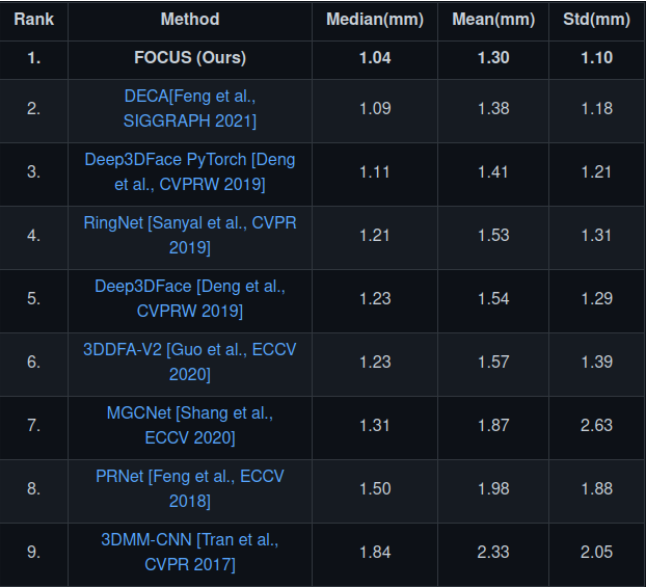
\includegraphics[width=1\linewidth]{now}
 		\label{fig:now}
 		\caption{NoW Challenge benchmark eredményei
 			Forrás: https://github.com/unibas-gravis/Occlusion-Robust-MoFA}
 	\end{figure}
 	
 	\subsection{Értékelés}
 	
 	Mint láthatjuk a fent említett megközelítések mind kiváló eredményeket
 	nyújtanak, de megfigyelhetjük hogy a két munkának a szerzői teljesen
 	különböző motivációval rendelkeztek.
 	A $DECA$ főbb motivációja az emberi arc részleteinek megőrzése valamint az arc realisztikus animálhatósága. A
 	$FOCUS$ célja pedig egy gyors modell kialakítása volt, amely korábbi
 	munkákhoz képest jobban kezeli a kitakarásokat. A mi célunk, egy olyan
 	animálható modell kialakítása, amely képes megőrízni a részleteket. Emellett képes konzisztens mükődést nyújtani súlyos kitakarások jelenlétében is.
 	
 	Tehát a tervezett modell, amit a későbbiekben részletesebben
 	megvizsgálunk kettő egymást támogató hálózatból áll. Egyik fő épitőeleme a
    $DECA$ alapján készített rekonstrukciós hálózat. A másik,
 	a $FOCUS$ megközelítésében implementált szegmentációs hálózat. E két
 	hálózaton egy EM típusú stratégiát alkalmazunk a tanítási folyamat
 	során.
 	
 
	 \section{3D arcmodell konstruálása}
	 \label{3d}
	 \cite{survey} A 3D-s arcok legelterjedtebb statisztikai modellje a 3D Morphable Models (3DMM), amelyet Blanz és Vetter \cite{blanzvetter} mutatott be a közösségnek. Bernhard és tsai. \cite{3dmm} munkája alapján a 3D Morphable Face Model egy generatív modell az arcformára
	 és a megjelenés modellje, amely két kulcsfontosságú ötleten alapul:
	 
	  Először is, minden arc
	 sűrű pont-pont megfeleltetésben van, amelyet általában egy regisztrációs eljárás során egy sor példaarcon állítanak elő, majd
	 a további feldolgozási lépések során is megmarad.Ennek a megfeleltetésnek köszönhetően az arcok lineáris kombinációi definiálhatók egy értelmes módon, morfológiailag valósághű arcokat (morfokat) létrehozva.
	 
	 
	 A második ötlet az arc alakjának és színének szétválasztása, és ezek függetlenítése a külső tényezőktől, például a megvilágítástól és a kamera paraméterektől.
	 
	  A \textit{morphable} modell magában foglalhat egy statisztikai modellt
	 az arcok eloszlásáról, amely egy főkomponens elemzés az eredeti munkában.
  Egy lineáris
alteret határoznak meg az alakzat és a textúra reprezentálására főkomponens elemzés \cite{PCA} segítségével, és bemutatják, hogyan lehet a modellt az adatokra illeszteni. 

	 \subsection{Arcképfelvétel}
	  Minden 3D statisztikai arcmodell legfontosabb összetevője a 3D alakzatok reprezentatív készlete a megfelelő megjelenési adatokkal együtt. A mintakészlet létrehozásának tipikus módja, hogy az adatokat a valós világból kapjuk meg. Ebben a szakaszban rövid áttekintést adunk a különböző megközelítésekről, amelyeket az arcadatok, valamint az arcképek adatainak megszerzésére használatosak \cite{3dmm}.
	  
	 A bemeneti adathalmazok létrehozása a 3DMM-ek számára kontrollált körülmények között történő felvételre korlátozódnak szemben a nagyobb kihívást jelentő kontrollálatlan felvételekkel.
	 
	 Megjegyzendő, hogy a kontrollált 3D arcfelvétel nem mindig szükséges. Voltak kísérletek arra, hogy a 3DMM-eket közvetlenül képekből tanulják meg. Például Cashman és Fitzgibbon munkája 2012-ben \cite{dolphins} és a legmodernebb mélytanuláson (\textit{deep learning}) alapuló módszerek egyszerre tanulnak 3DMM-et és regresszió-alapú illesztést 2D-s tanítási adatokból.
	 
	 \subsection{Alakfelvétel}
	 A háromdimenziós forma vitathatatlanul a 3DMM legfontosabb összetevője \cite{3dmm}. Az alakzat ábrázolásának kérdése
	 a 3DMM-ek összefüggésében nem került széles körben figyelembe vételre.
	 
	  Messze a
	 leggyakrabban használt reprezentáció a háromszögháló. Vannak ritka kivételek, de ebben a munkában ezeket nem fogjuk megemlíteni.
	 
	  A háromszöghálós reprezentáció sűrű megfeleltetéssel megköveteli, hogy minden minta azonos topológiát mutasson, és hogy a csúcsok minden mintán ugyanazt a szemantikai pontot kódolják. A minták közötti megfelelés megállapítása önmagában is kihívást jelentő téma. Ebben a szakaszban a nyers 3D adatokra összpontosítunk.
	
	
	\subsubsection{Statisztika alapú modell illesztési módszerek}
	A statisztikai 3D arcmodell \cite{survey} a legnépszerűbb módszer az előzetes információ hozzáadására, mivel ezek kódolják az arc geometriai variációit, esetleg a megjelenéssel együtt.
	
	 Az ilyen modellek tartalmaznak egy átlagos arcot, valamint annak geometriájának és az arcmintázatának a variációit és a megjelenését.
	 
	  3D arcmodell illesztése fényképre
	a modell paraméterein kívül,
	a 3D póz és a megvilágítás meghatározásával történik úgy, hogy
	az eredményül kapott 3D-s arc képsíkjába történő vetülete
	a lehető legjobban hasonlítson az adott képhez.
	
	\subsubsection{Geometriai módszerekhez}
	A geometriai módszerek \cite{3dmm} közvetlenül becslik egy alakzat 3D-s koordinátáit vagy ugyanazon felület megfigyelésével
	két vagy több nézőpontból (ebben az esetben a kihívás a megfelelő pontok azonosítása a képek között), vagy pedig egy vetített minta megfigyelésével (ebben az esetben a kihívás az ismert minta és a róla készült vetület kép közötti megfeleltetés azonosítása).
	
	 A módszerek vagy aktívnak tekinthetők, azaz fényt
	vagy más jeleket sugároznak, vagy passzívak.
	
	
	A lézerszkennerek, a \textit{Time-of-Flight} érzékelők és a strukturált fényrendszerek \textit{aktív} rendszerek, míg a több nézetből álló fotogrammetria \textit{passzív} alternatíva.
	
	\subsubsection{Fotometrikus módszerek}
	A fotometrikus módszerek \cite{3dmm} jellemzően a felület orientációját becslik, amelyből integrálással vissza lehet nyerni a 3D alakot.
	
	 A kihívás itt az, hogy olyan modelleket válasszunk, amelyek pontosan megragadják a felszín reflexiós tulajdonságait, valamint elegendő mérési eredményt kapjunk ahhoz, hogy e modellek invertálása jól megoldható legyen. 
	 
	 A geometriai módszerekhez képest a fotometriai módszerek
	 jellemzően nagyobb alaki részletességet kínálnak, és nem függnek a
	 összeilleszthető jellemzők meglététől
	(tehát sima, jellegtelen felületek esetén is alkalmazhatóak), de gyakran szenvednek alacsony frekvenciájú torzításoktól a rekonstruált képekben
	a fényvisszaverő képesség és a megvilágítás modellezési hibái miatt.
	
	
	A fotometrikus sztereó \cite{photometric} a felszín normálisa adja meg minden egyes képpontnál a jelenet rögzített pozícióból történő megfigyelésével, legalább három különböző megvilágítási körülmény között.
	
	 A szükséges képkockák számát spektrális multiplexálással lehet csökkenteni \cite{multiplex}.
	
	\subsubsection{Hibrid módszerek}
	A hibrid módszerek \cite{3dmm} a
	geometriai és a fotometriai módszerek kombinációja. 
	
	Csökkentik a
	a fotometriai módszereknél jellemzően jelenlévő alacsony frekvenciájú torzítást, és
	növelik a nagyfrekvenciájú részleteket a geometriai módszerekhez képest. 
	
	Diego Nehab és tsai. \cite{hibrid} javaslata egy olyan módszer, amely helymeghatározó információk alacsony frekvenciáját egyesíti a felszíni normálisok magas frekvenciájával. 
	A módszer különösen hatékony, mivel csak egy lineáris egyenletrendszer megoldása szükséges. 

    \subsection{FLAME modell}

    Mint ahogyan már említettük, Blanz és Vetter javasolták az első általános 3D modellt \cite{3dmm}, ami szkennelt adatokból tanult. Meghatároztak egy lineáris alteret az alak és a textúra reprezentálására főkomponens analizis (PCA) segitségével. Illetve bemutatják hogyan kell a modellt az adatokhoz illeszteni. A modell 200 fiatal, többnyire kaukázusi felnőtt fejének szkenneléséből épült fel. A modellnek jelentős hatása volt mivel nyilvánosan elérhető további kutási munkákhoz, mint például a Basel Face Model.

    A FLAME modell egy statisztikai fejmodell \cite{flame}, ami pontosabb és kifejezőbb mint a korábbi fej- és arcmodellek, miközben kompatibilis marad a szabványos grafikus szoftverekkel.
    A már meglévő modellekkel ellentétben a FLAME explicit módon modellezi a fej tartását és a szemgolyó forgását.

    A FLAME egyesíti a különálló lináris identitásalak és kifejezés tereket $linear$ $blend$ $skinning$-gel (LBS) és a pózfüggő korrektív $blendshape$ alakzatokat, annak érdekében, hogy
    a nyak, az állkapocs és a szemgolyók mozgathatóak legyenek. Adott arc identitás $\beta ∈ R^{|\beta|}$, póz $\theta \in R^{3k+3}$ (ahol $k = 4$ a nyak, állkapocs, és szemgolyók ízületeinek száma), és arckifejezés $\psi \in R^{|\psi|}$ paraméterek mellett, a FLAME egy $n = 5023 $ csúcspontot tartalmazó archálót ad kimenetül.
    A modell a következőképpen van definiálva: 
    \begin{equation*}
        M (\beta, \theta, \psi) = W (T_{p}(\beta, \theta, \psi), J(\beta), \theta, W)
    \end{equation*}
    ahol, a $blendskinning$ függvény $W (T, J, θ, W)$ elforgatja a 
    $T \in R^{3n}$ csúcsait a $J \in R^{3k}$ ízületek körül, lineárisan finomítva a $W \in R^{k\times n}$
    keverési súlyokkal. A $J$ ízületi helyek a $\beta$ identitás függvényeként definiálhatók.
    Továbbá, 
    \begin{equation*}
        T_{p}(\beta, \theta, \psi) = T + B_{S}(\beta, S) + B_{P}(\theta, P) + B_{E}(\psi, E)
    \end{equation*}
     jelöli a $T$ minta átlagát ”nullpózban” a hozzáadott alak blendshape-ekkel $B_{S} (\beta, S) : R^{|\beta|} \Rightarrow R^{3n}$, pózkorrekciókkal $B_{P}(\theta, P) : R^{3k+3} \Rightarrow R^{3n}$, valamint kifejezés blendshape-ekkel $B_{E}(\psi, E) : R^{|\psi|} \Rightarrow R^{3n}$, a megtanult identitás-, póz- és kifejezésalapokkal (lineáris alterekkel) $S, P$ és $E$. \\

    A legtöbb korábbi módszer figyelmen kívül hagyta a szemeket a
    hozzáigazítás során. Ez torzítja a szemhéjakat és jelentős fotometriai hibákat okoz a szemek régiójában. Következésképpen szemgolyókat adtak hozzá a hálóhoz és bizonyították, hogy ez segíti az igazítási folyamatot.

    Egyik fő szempont, hogy kutatásunkban a FLAME modellt használjuk, az hogy a FLAME betanított modelljeit kutatási célokra nyilvánosan hozzáférhetővé tették, valamint a modell segítségével animálható 3D arcok készíthetőek.

    \subsection{Linear Blend Skinning (LBS)}
    A Linear Blend Skinning (LBS) a számítógépes grafikában használt technika, amely egy 3D objektumot egy csontok halmazának mozgása alapján deformál. 
Általában a 3D animációban használják a karakterek vagy tárgyak valósághű mozgásának létrehozására.

Az LBS-t a 3D arcmodell deformálására használjuk az arc tájékozódási pontok vagy a 2D tájékozódási pont detektor által megjósolt tájékozódási pontok mozgása alapján.
 A folyamat a következő lépésekből áll:

\begin{enumerate}
    \item \textbf{Súlyok hozzárendelése minden egyes csúcshoz}: 
    
    Ez határozza meg, hogy az egyes csontok milyen mértékben befolyásolják az egyes csúcsokat. 
	A súlyok jellemzően olyan értékek halmazaként jelennek meg, amelyek összege minden egyes vertex esetében 1. A DECA-ban ezeket a súlyokat a Softmax nevű módszerrel számítják ki.

    \item \textbf{Az átalakított csúcspont pozíciójának kiszámítása}: 
    
    Az egyes csúcspontok pozícióját az egyes csontok pozíciója és orientációja alapján transzformáljuk. 
	Ez úgy történik, hogy a csúcspont pozícióját megszorozzuk az egyes csontokra kiszámított transzformációs mátrixszal. 
	A csúcspont végső pozíciója az összes transzformált pozíció összege, az egyes csontokhoz rendelt súlyokkal súlyozva.

    \item \textbf{A deformáció alkalmazása}: 
    
    A transzformált csúcsokat a 3D arcmodell deformálására használjuk. A deformált modellt ezután rendereljük a végső kimenet létrehozásához.
\end{enumerate}

Az LBS egy egyszerű és hatékony technika, amellyel valós idejű, realisztikus animációk hozhatók létre. 
Azonban vannak bizonyos korlátai, például nem képes kezelni az összetett deformációkat. 
A DECA-ban az LBS-t más technikákkal, például a BlendShape animációval kombinálják, hogy valósághűbb és pontosabb arcanimációkat hozzanak létre.

 
	\section{Neurális hálózatok}
	\subsection{Neurális hálózat}
    Ebben a fejezetben Abraham és tsai. munkája alapján bemutatjuk a neurális hálózatok működését.
    
	\label{NN}
	Az emberi agy bizonyítja a hatalmas neurális hálózatok létezését, amelyek sikeresen végeznek el kognitív, észlelési és irányítási feladatokat. Ilyen számításigényes feladat például az arcfelismerés, a beszéd és a testmozgás. Az agy hatékonyan kihasználja a masszív párhuzamosságot, számítási struktúrája nagymértékben párhuzamos és jó információfeldolgozási képességgel rendelkezik.
	
	Az emberi agy több, mint 10 milliárd egymással összefüggő neuron gyűjteménye. Mindegyik neuron egy sejt \ref{fig:neuron1}, amely biokémiai reakciókat használ az információ fogadáshoz, feldolgozáshoz és továbbításhoz.
	
	Az idegrostok faszerű hálózatai, az úgynevezett dendritek kapcsolódnak a sejttesthez, ahol a sejtmag található. A sejttestből egyetlen hosszú rost nyúlik, melyet \textit{axon}nak neveznek. Az \textit{axon} szálakra és alszálakra ágazik, majd szinapszisain keresztül kapcsolódik más neuronokhoz. Az itt létrejövő szinaptikus kapcsolat erőssége határozza meg az emberi agy tanulását\cite{ann} .
	
	A jelek átvitele egyik neuronról a másikra a szinapszisoknál egy összetett kémiai folyamat, amelyben specifikus közvetítő anyagok szabadulnak fel a kapcsolódási pont küldői oldalán. A folyamat hatására a fogadó sejtben emelkedik vagy csökken az elektromos feszültség.
	\begin{figure}[h]	
		\centering
		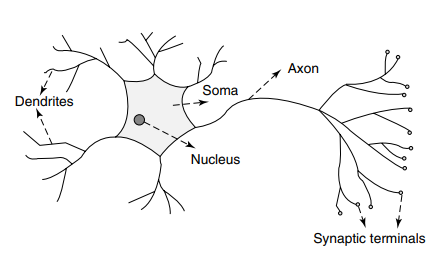
\includegraphics[width=1\linewidth]{neuron1}
        \label{fig:neuron1}
		\caption{Neuron felépítése. 
			Forrás:\cite{ann}}
	\end{figure}
	\newpage
	\subsection{Mesterséges neurális hálózatok}
	A mesterséges neurális hálózatok (ANN-artificial neural networks) az előző fejezetben [\autoref{NN}] említett fejlettebb élő szervezetek agyát alkotó neuronokról kapták nevüket. 
	
	Mint azt \textit{Abraham} és tsai. \cite{ann} is említik, a neurális hálózatok alapvető feldolgozási elemeit mesterséges neuronoknak nevezzük, vagy csak egyszerűen neuronoknak vagy csomópontoknak. A neuron leegyszerűsített matematikai modelljében a szinapszisok hatásai kapcsolati súlyokkal vannak reprezentálva, amelyek szabályozzák a bemeneti jelek hatását.
	
	 A neuronok által mutatott nonlineáris karakterisztikát átviteli függvény segítségével ábrázoljuk. A neuron impulzusát ezután a bemeneti jelek súlyozott összegeként számíthatjuk ki az átviteli függvénnyel transzformálva.
	 
	  Egy mesterséges neuron tanulási képessége a súlyok megfelelő beállításával érhető el egy választott tanító algoritmus felhasználásával.
	\newline
	\newpage
	Egy tipikus mesterséges neuron és egy többrétegű neurális hálózat modellezése a \ref{fig:fig2}. ábrán látható. A \ref{fig:fig2}. ábrán szerint, ahogy a nyilak is mutatják, az $x_{1},...,x_{n}$ bemenetekről érkező jeláramlás egyirányúnak tekinthető csakúgy, mint a neuron kimeneti jelfolyama. A neuron kimeneti jelét \textit{O} a következő összefüggés adja:
	\begin{mdframed}
	\begin{align}
		&O = f(net) = f(\sum{j=1}^{n}w_{j}x_{j}) 
		\intertext{ahol $w_{j}$ a súly vektor és $f(net)$ az \textit{aktivációs} (átviteli) függvény. A \textit{net} változó a súly és a bementi vektorok skaláris szorzataként definiálható,}
		&net = w^{T}x = w_{1}x_{1} + ... + w_{n}x_{n}
		\intertext{ahol T egy mátrix transzponálását jelöli, és a legegyszerűbb esetben a kimeneti érték \textit{O} kiszámítható, mint}
		&O = f(net) = 
		\begin{cases}
			1,; ha ; w^{T}x ; \geq ; \theta \
			0, \text{különben} \
		\end{cases} \
	\end{align}
	ahol $\theta$-t \textit{küszöbszintnek} (threshold) nevezzük. Ezt a típusú aktivációs függvényt \textit{küszöb aktivációs függvénynek} nevezzük.
	
	\end{mdframed}
	
	
	\begin{figure}[h]%
		\centering
		\subfloat[\centering Mesterséges neuron]{{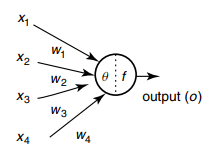
\includegraphics[width=5cm]{artificialNeuron} }}%
		\qquad
		\subfloat[\centering Többrétegű neurális háló]{{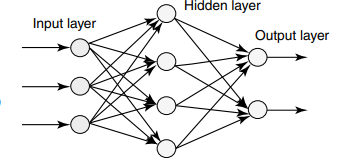
\includegraphics[width=5cm]{multilayered} }}%
		\caption{Mesterséges neuron felépítése és egy többrétegű neurális háló \newline\centering Forrás: \cite{ann}}%
		\label{fig:fig2}%
	\end{figure}
	\newpage
	A \textit{küszöbfüggvényhez} hasonlóan más aktivációs függvényekkel is előállítható az adott neuron bemenetre kapott válasz. Ilyen függvények a 
	\begin{itemize}
		\item lineáris,
		\item szigmoid,
		\item tangens hiperbolikusz.
	\end{itemize}

	\begin{figure}[h]	
		\centering
		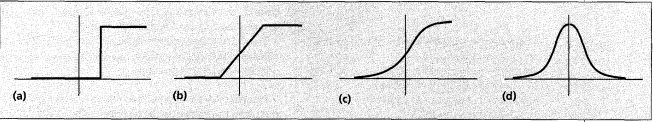
\includegraphics[width=1\linewidth]{fuggvenyek}
		\caption{(a) küszöbfüggvény, (b) lineáris, (c) szigmoid, (d) Gauss 
			\newline\centering Forrás:\cite{ann2}}
		\label{fuggvenyek}
	\end{figure}
	
	\begin{mdframed}
	Ma az egyik leggyakrabban használt aktivációs függvény a szigmoid \cite{ann4}, melyet a következő képlettel határoznak meg:
	\begin{align}
		&y = \frac{1}{1 + e^{-(a - \theta)b}}
	\end{align}
	ahol \textit{a} az aktiválás, \textit{b} pedig a görbe alakját szabályozza.
	\end{mdframed}
	
	\subsection{Neurális hálózat architektúra}
	
	Bár a mesterséges neuron működési elvei és 
	egyszerű szabályrendszere elsőre talán nem tűnik érdekesnek, azonban e modellek teljes potenciálja és számítási teljesítménye akkor kel életre, 
	amikor mesterséges neurális hálózatokká
	kezdjük őket összekapcsolni \ref{fig:fig2}. ábrán. 
	Ezek a mesterséges neurális hálózatok 
	kihasználják az egyszerű tényt, 
	hogy a komplexitás néhány alapvető
	szabályból tud növekedni.
	
	A mesterséges neurális hálózatok 
	képesek komplex, valós problémák megoldására azáltal
	, hogy 
	alapvető építőelemeikben (\textit{mesterséges neuronok}) feldolgozzák az információt nemlineáris,
	elosztott, párhuzamos és lokális módon.
	
	Krenker és tsai. 
	\cite{krenker} munkája alapján az egyes mesterséges 
	neuronok összekapcsolásának módját 
	\textit{topológiának}, \textit{architektúrának} 
	vagy \textit{gráfnak} nevezzük. A tény, 
	hogy az összekapcsolás
	számos lehetséges módon történhet több alkalmazható topológiát eredményez, amelyek két fő csoportra bonthatók. 
	
	A \ref{fig:topologies}. ábra ezt a két topológiát mutatja. Az ábra bal oldala egy egyszerű feedforward topológiát ábrázol, ahol az információ a bemenetekről kimenetekre áramlik egyirányúan. Az ábra jobb oldala pedig egy egyszerű rekurzív (\textit{recurrent}) topológiát ábrázol, ahol az információ egy része nem csak egy irányban áramlik a bemenetről a kimenetre, hanem ellenkező irányban is.

	Fontos megemlíteni, hogy a mesterséges neurális hálózat könnyebb kezelése és matematikai leírása érdekében az egyes neuronokat rétegekbe soroljuk. A \ref{fig:topologies}. ábrán láthatjuk a bemeneti, a rejtett és a kimeneti réteget.
	\begin{figure}[h]	
		\centering
		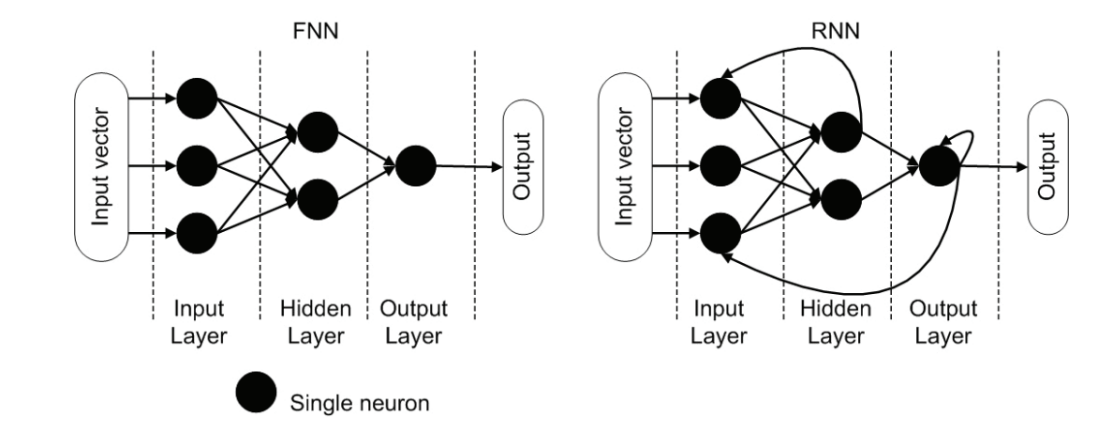
\includegraphics[width=1\linewidth]{topologies}
        \label{fig:topologies}
		\caption{Feed-forward (FNN) és recurrent (RNN) \newline\centering  neurális hálózati topológiák. 
			Forrás:\cite{krenker}}
	\end{figure}

	A háló input rétegében minden neuron kapcsolatban áll a \textit{rejtett} (köztes) réteggel, így tovább adhatja a bemenetként kapott adatokat. A bemeneti réteg neuronjai súlyozott szinapszisokkal kapcsolódnak a belső rétegekhez.\\
	
	A mesterséges neurális hálózat 
	topológiájának kiválasztásával és 
	felépítésével még csak a feladataink 
	felét fejeztük be mielőtt a hálót az 
	adott probléma megoldására használhatnánk.
	Csakúgy, mint a biológiai neurális hálózatoknak
	is meg kell tanulniuk a megfelelő válaszokat különböző környezeti bemenetekre, a mesterséges neurális hálózatoknak is pontosan ezt kell tenniük.
	
	
	A következő lépés tehát, hogy \textit{betanítsuk} a mesterséges neurális hálózatot a helyes válaszokra.
	Erre négy lehetőségünk van:
	\begin{itemize}
		\item a felügyelt
		\item a felügyelet nélküli
		\item a megerősítéses
		\item és a hibrid
	\end{itemize}
	tanulás.
	
	 Függetlenül attól, hogy melyik módszert választjuk, a tanulás feladata, hogy a tanulási adatok alapján beállítsuk a súlyok és az előfeszítések értékeit, hogy minimalizáljuk a 
	költségfüggvényt.
	
	\subsection{Neurális hálók tanítása}
    Ebben a fejezetben \cite{krenker} és tsai. munkája alapján mutatjuk be a nerális hálózatok tanítási módszereit.
 
	A tanulási folyamat \cite{ann2} az ANN kontextusában a
	hálózat architektúrája és a kapcsolati súlyok frissítéseként értelmezhető annak érdekében, hogy a háló hatékonyan tudjon elvégezni egy adott feladatot.
	A hálózatnak a rendelkezésre álló tanító mintákból kell megtanulnia a kapcsolati súlyokat. A teljesítmény idővel javul a súlyok iteratív frissítésével.
	Az ANN-eket automatikus, példákból való tanulása teszi 
	vonzóvá és érdekessé. Szakértők által definiált szabályok helyett az ANN-ek a mögöttes szabályokat tanulják meg (pl. bemeneti-kimeneti kapcsolatokat) a megadott reprezentatív példák gyűjteményéből.
	
	\subsubsection{Felügyelt tanulás (\textit{supervised learning})}
	
	A felügyelt tanulás egy olyan gépi tanulási (\textit{machine learning}) technika, amely egy mesterséges neurális hálózat paramétereit tanítási
	adatokból állítja be. A tanuló ANN feladata, hogy beállítsa paramétereinek értékét bármely érvényes bemeneti értékre, miután látta a kimeneti értéket.
	A képzési adatok a bementi és a kívánt kimeneti értékek párjaiból állnak, amelyeket adatvektorokban ábrázolnak.
	
	
	A felügyelt tanulást \textit{klasszifikációnak} is nevezhetjük, ahol \textit{osztályozók} széles skálája áll rendelkezésünkre, amelyek mindegyikének megvannak az erősségei és gyengeségei.
	A felügyelt tanulás egy
	adott problémájának megoldásához különböző lépéseket kell figyelembe venni.
	
	 Az első lépésben meg kell határoznunk a tanítási minták típusát. A második
	lépésben olyan tanítási adathalmazt kell gyűjtenünk, amely kielégítően leírja az adott problémát.
	A harmadik lépésben az összegyűjtött tanítási adathalmazt
	olyan formában kell leírnunk, amely érthető a kiválasztott ANN számára. A negyedik lépésben elvégezzük
	a tanítást. Ezután tesztelhetjük a tanult ANN teljesítményét a teszt (validációs) adathalmazzal.
	A validációs adathalmaz olyan adatokból áll, amelyeket a tanulás során nem vezettünk be a mesterséges neurális hálózatba.
	
	\subsubsection{Felügyelet nélküli tanulás (\textit{unsupervised learning})}
	
	A felügyelet nélküli tanulás egy olyan gépi tanulási (\textit{machine learning}) technika, amely egy ANN paramétereit megadott adatok és egy minimalizálandó 
	költségfüggvény alapján állítja be. A költségfüggvény bármilyen függvény lehet, amit a feladat határoz meg.
	
	
	Felügyelet nélküli tanulást leginkább olyan alkalmazásokban használnak, amelyek a becslési problémák körébe tartoznak, mint például a statisztikai modellezés, filterezés és a klaszterezés. A felügyelet 
	nélküli tanulás során arra törekszünk, hogy meghatározzuk, hogyan szerveződnek az adatok. Ez a felügyelt és a megerősítéses tanulástól abban különbözik, hogy az ANN csak \textit{címkézetlen} mintákat kap. A felügyelet nélküli tanulás egyik gyakori formája a klaszterezés, ahol az adatokat hasonlóságuk alapján próbáljuk különböző klaszterekbe sorolni.
	
	\subsubsection{Megerősítéses tanulás (\textit{reinforcement learning})}
	
	A megerősítéses tanulás egy olyan gépi tanulási (\textit{machine learning}) technika, amely egy olyan
	mesterséges neurális hálózat paramétereit állítja be, ahol általában az adatok nincsenek előre megadva, hanem a környezettel való kölcsönhatásokból generálódnak. A megerősítéses tanulás azzal foglalkozik, hogy egy mesterséges neurális hálózatnak hogyan kellene viselkednie egy adott környezetben annak érdekében, hogy maximalizálja a hosszú távú 
	eredményeket.
	
	Miután a maximalizálandó visszatérési függvényt meghatároztuk, a megerősítéses tanulás számos algoritmust használ a maximális visszatérést eredményező szabályok meghatározására. Az első lépésben egy naiv \textit{brute force} algoritmus kiszámítja a \textit{visszatérési függvény}t minden lehetséges szabályhoz és kiválasztja azt, amelyik a legnagyobb visszatéréssel rendelkezik. Ennek az algoritmusnak nyilvánvaló gyengesége a rendkívül magas vagy akár végtelen számú lehetséges szabály esetében rejlik. Ez a gyengeség kiküszöbölhető érték függvényes megközelítésekkel vagy közvetlen szabály becslésekkel. Az értékfüggvényes megközelítések megpróbálnak
	egy olyan szabályrendszert találni, amely maximalizálja a visszatérést.
	
	Ezek a módszerek konvergálnak a helyes becslésekhez egy rögzített szabály esetén, és az optimális szabály megtalálására is használhatóak. Az értékfüggvényes megközelítéshez hasonlóan a közvetlen szabály becslés is képes megtalálni az optimális szabályt.

    \subsubsection{Átviteli tanítás}
    
     A hagyományos gépi tanulási módszerek egyik feltételezése, hogy a tanítási és tesztelési adatok ugyanabból a tartományból származnak, így a bemeneti jellemzőtér és az adatok eloszlási jellemzői megegyeznek. Néhány valós gépi tanulási forgatókönyvben azonban ez a feltételezés nem áll fenn. Vannak olyan esetek, amikor a képzési adatok gyűjtése drága vagy nehézkes. Ezért nagy teljesítményű tanulók létrehozására van szükség, amelyeket különböző tartományokból könnyebben beszerezhető adatokkal tanítanak. Ezt a módszert átviteli tanulásnak nevezzük \cite{tl}.

     Az átviteli tanítás alapvető célja a modell fejlesztésének felgyorsítása egy meglévő modellből kiindulva és annak tovább hangolása a specifikus problémára.
 
	\subsection{Konvolúciós neurális hálózatok}
	\begin{figure}[h]	
		\centering
		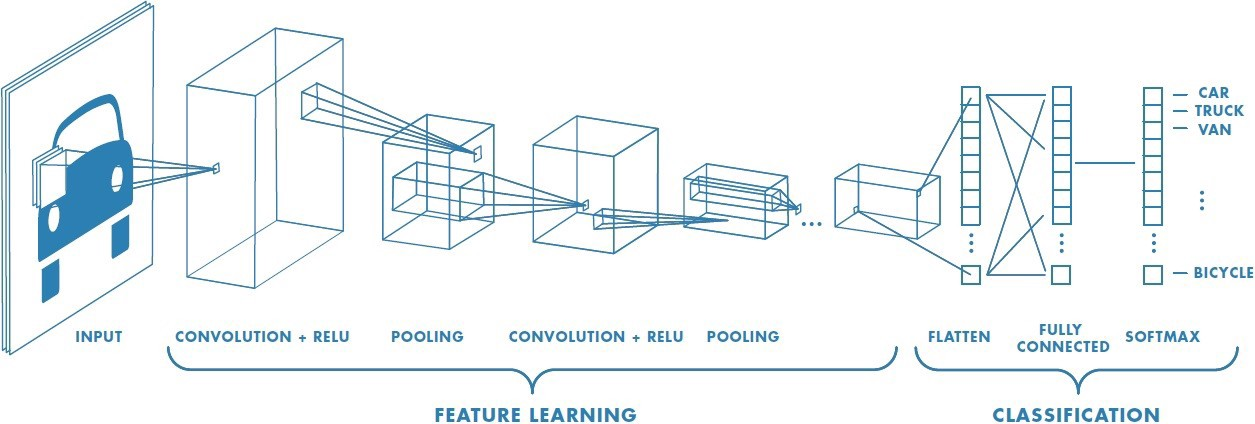
\includegraphics[width=1\linewidth]{CNN}
        \label{fig:cnn}
		\caption{CNN(Convolutinal Neural Network)}
	\end{figure}
	Indolia és tsai. \cite{CNN} értelmezésében a konvolúciós neurális hálózat (CNN) egy
	mélytanulási megközelítés, amelyet széles körben használnak komplex problémák megoldására és felülmúlja a hagyományos gépi
	tanulási megközelítéseket.
	
	A konvolúciós neurális hálózat mély feed-forward architektúrával rendelkezik, és jobban képes általánosítani, mint a teljesen összekapcsolt rétegekkel rendelkező hálózatok.
	
	A CNN, mint a hierarchikus jellemző detektorok biológiailag inspirált koncepciója, képes nagymértékben megtanulni
	absztrakt jellemzőket és hatékonyan képes azonosítani az objektumokat.
	
	A CNN-t az alábbi előnyökkel rendelkezik más klasszikus modellekkel szemben:
	
	  A CNN-ek alkalmazásának legfőbb előnye a súlymegosztás koncepciójában rejlik
	, amelynek köszönhetően a betanítandó paraméterek száma jelentősen csökken, ami jobb általánosításhoz vezet. 
	A kevesebb paraméter miatt a CNN egyszerűen betanítható, és nem szenved túlillesztéstől(overfitting).
	
	
	Másodszor, az osztályozási szakasz beépül a jellemző kinyerési szakaszba. Mindkét szakasz használ tanulási folyamatot.
	
	
	Harmadszor, a mesterséges neurális hálózat általános modelljeinek felhasználásával nagy hálózatokat sokkal nehezebb megvalósítani,
	mint CNN-ben.
	
	
	A CNN-eket széles körben használják különböző területeken figyelemreméltó
	teljesítményüknek köszönhetően, mint például a képosztályozás, a tárgyak felismerése, az arcfelismerés, a beszéd
	felismerés, járműfelismerés stb.
	
	\subsection{A konvolúciós neurális hálózat általános modellje}
    Ebben a fejezetben Indolia és tsai. \cite{CNN} munkéja alapján bemutatjuk a CNN-ek általános modelljét.
 
	\subsubsection{Általános modell}
	Az ANN általános modellje egyetlen bemeneti és kimeneti réteggel,
	valamint több rejtett réteggel rendelkezik.
	
	Egy bizonyos 
	neuron fogadja az X bemeneti vektort, és Y kimenetet állít elő azáltal,
	hogy valamilyen F függvényt hajt végre rajta az alábbi általános egyenlet alapján (\ref{eq1}).
	\begin{mdframed}
	\begin{equation}
    \label{eq1}
			F(X, W) = Y
	\end{equation}
	,ahol W a súlyvektor, amely a két neuron közötti összeköttetés erősségét jelöli két szomszédos réteg között.
 	\end{mdframed}

	A kapott súlyvektor most már felhasználható a képosztályozáshoz.
	
	Jelentős mennyiségű irodalom létezik a képek pixelalapú osztályozásával
	kapcsolatban, azonban az olyan kontextuális információk, mint a kép alakja vagy 
	a kép formája jobb eredményt adnak.
	
	A CNN a kontextuális információkon alapuló osztályozási képessége miatt kap egyre nagyobb figyelmet.\\
	
	
	A CNN általános modellje négy komponensből áll, nevezetesen 
	\begin{itemize}
		\item konvolúciós réteg
		\item pooling réteg
		\item aktivációs függvény
		\item teljesen összekapcsolt réteg
	\end{itemize}
	Az egyes komponensek működését az alábbi [\ref{fig:cnnelem}.] ábra szemlélteti.
	
	\begin{figure}[h]	
		\centering
		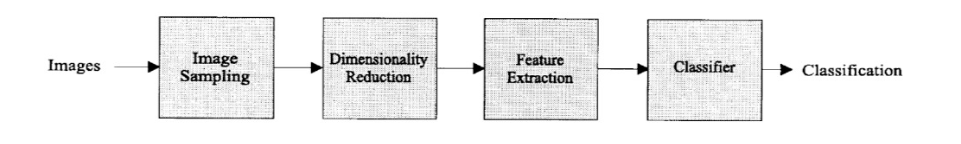
\includegraphics[width=1\linewidth]{element}
        \label{fig:cnnelem}
		\caption{\cite{CNN} A CNN elemi összetevői}
	\end{figure}

	
	\subsubsection{Konvolúciós réteg}
	
	Az osztályozandó képet a bemeneti rétegnek adjuk meg, a kimenet pedig az előre megjósolt osztálycímke, amelyet a képből kinyert jellemzők alapján számítunk ki.
	
	
	A következő rétegben lévő egyes neuronok az azt követő rétegben lévő neuronokhoz kapcsolódnak. Ezt a helyi korrelációt receptív mezőnek nevezzük.
	
	
	A bemeneti kép lokális jellemzőit a receptív mező segítségével nyerjük ki. Az előző rétegben egy adott régióhoz tartozó neuron receptív mezeje egy súlyvektort alkot, amely a sík minden pontján egyenlő marad, ahol a sík a következő rétegben lévő neuronokra utal. Mivel a síkban lévő neuronok azonos súlyokkal rendelkeznek, így a különböző helyeken előforduló hasonló jellemzők a bemeneti adatokon belül felismerhetők.
	
	\begin{figure}[h]	
		\centering
		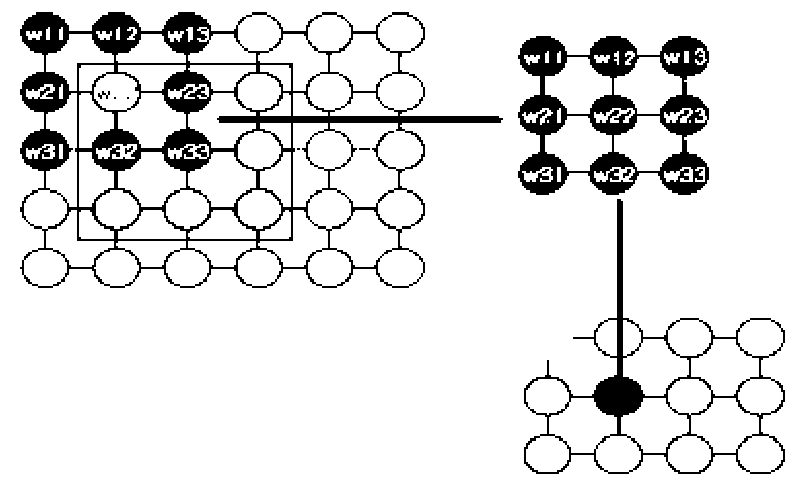
\includegraphics[width=0.7\linewidth]{receptiv}
		\caption{\cite{CNN} Az adott neuron receptív mezeje a következő rétegben}
	\end{figure}
		\newpage
	A súlyvektor, más néven szűrő vagy kernel a bemeneti vektoron csúszik át a \textit{featuremap} létrehozásához.
	A szűrő vízszintes és függőleges irányú csúsztatásának módszerét nevezzük konvolúciós műveletnek. A helyi receptív mező jelensége miatt a betanítható paraméterek száma jelentősen csökken.
	
	A következő rétegben az (i,j) helyhez tartozó $A_{ij}$ kimenet konvolúciós
	művelet alkalmazása után kerül kiszámításra az alábbi képlet segítségével:
	\begin{mdframed}
	\begin{align}
		a_{ij} = \sigma((W * X)_{ij} + b)
	\end{align}
	, ahol X a rétegnek adott bemenet, W a bemeneten áthaladó szűrő vagy kernel,
	b az eltolás, * a 
	a konvolúciós műveletet, és $\sigma$ a hálózatba bevezetett non-linearitást jelöli.
	\end{mdframed}
	
	\subsubsection{Összevonó réteg}

	A konvolúciós réteget összevonó (pooling) vagy 
	almintavételező (sub-sampling) \cite{CNN} réteg követi.
	A \textit{pooling} technika használatának fő előnye, hogy 
	jelentősen csökkenti a betanítható paraméterek számát,
	és bevezeti a fordítási invarianciát. 
	
	
	Az összevonás (\textit{pooling}) művelet elvégzéséhez kiválasztunk egy ablakot,
	és az abban az ablakban lévő bemeneti elemeket átadjuk
	egy összevonó (\textit{pooling}) függvénynek. a [8. ábrán] látható módon.
	
	\begin{figure}[h]	
		\centering
		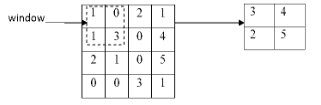
\includegraphics[width=0.7\linewidth]{pooling}
		\caption{\cite{CNN} 2 x 2 ablak kiválasztásával végzett összevonási művelet}
	\end{figure}
	
	\newpage
	
	A pooling függvény egy másik kimeneti vektort generál.
	
	
	Létezik néhány összevonási technika, mint például az átlagos összevonás (\textit{average pooling}). 
	és a \textit{max-pooling}, amelyek közül a \textit{max-pooling} a leggyakrabban használt módszer,
	mely jelentősen csökkenti a leképezés méretét.
	
	
	A hibák kiszámítása során a hiba nem terjed vissza a győztes egységre.
	
	\subsubsection{Teljesen összekapcsolt réteg}
	
	A teljesen összekapcsolt réteg \cite{CNN} hasonló a hagyományos modellek teljesen összekapcsolt hálózatához.
	
	
	Az első
	fázis kimenete (a konvolúciót és a összevonást ismétlődően tartalmazza) a teljesen összekapcsolt rétegbe kerül, és a súlyvektor és bemeneti vektor pontproduktumát számoljuk ki a végeredmény kiszámítása érdekében.
	
	
	A \textit{gradiens süllyedés}, más néven kötegelt módú tanulás vagy offline algoritmus, csökkenti a költségfüggvényt a költség becslésével egy teljes tanítói adathalmaz felett, és a paramétereket csak egy korszak után frissíti, ahol egy korszak a teljes adathalmaz átfutásának felel meg.
	Ez globális minimumokat eredményez, de ha a képzési adathalmaz mérete nagy, akkor a hálózat tanításához szükséges idő
	jelentősen megnő. A költségfüggvény
	\\
	csökkentésének ezt a megközelítését felváltotta a \textit{sztochasztikus gradiens süllyedés}.
	\subsubsection{Aktivációs függvény}
	
	
	Számos szakirodalom létezik, amely a hagyományos gépi tanulási algoritmusokban
	szigmoid aktivációs függvényt használ.
	A nemlinearitás bevezetése érdekében a Rectified Linear Unit (ReLU) \cite{CNN} használata jobbnak bizonyult az előbbinél
	két fő tényező miatt. 
	
	Először is, a ReLU parciális deriváltjának kiszámítása egyszerű. 
	Másodszor, miközben figyelembe vesszük
	a képzési időt mint az egyik tényezőt, a telítődő nemlinearitások, mint a szigmoid lassabbak, mint a nem telítődő nemlinearitások, mint a ReLU.
	 Harmadszor, ReLU nem engedi, hogy a gradiensek eltűnjenek, de a ReLU hatékonysága romlik, ha nagy gradiens áramlik át a hálózaton, és a súly frissítése miatt a neuron nem aktiválódik, ami a \textit{Dying ReLU} problémához vezet, amely egy jelentős probléma. 
	 
	 Ez a probléma megoldható a \textit{Leaky ReLU} segítségével, ha $x>0$, a függvény aktiválódik.
	mint $f(x)= x$, ha pedig $x<0$, akkor a függvény $\alpha x$-ként aktiválódik, ahol $\alpha$ egy kis konstans.

    \subsection{Reziduális Neurális Hálózatok}
    
    \begin{figure}[h]	
 		\centering
 		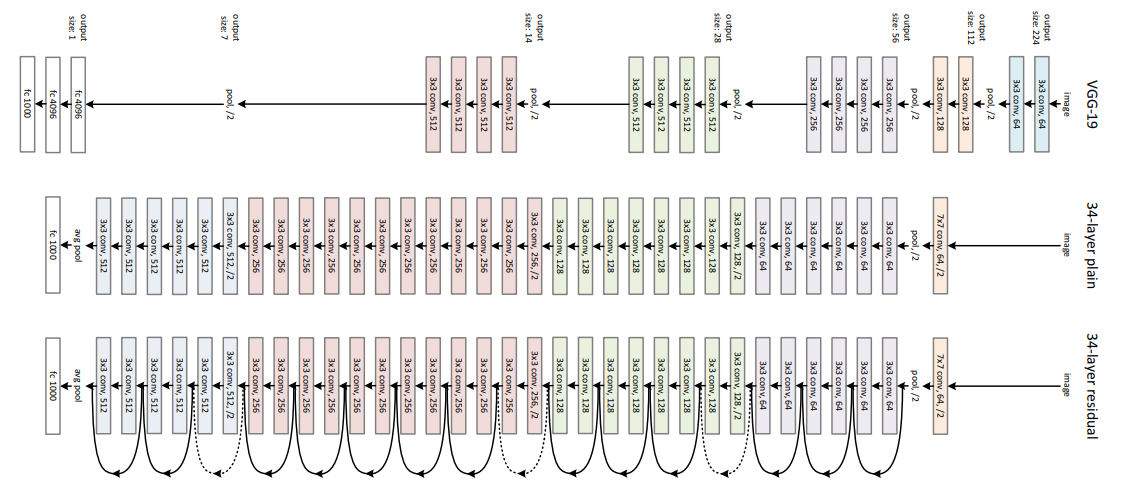
\includegraphics[width=1\linewidth]{ResNet}
 		\caption{ResNet architektúrák felépítése. (felülről a 3.)
 			Forrás:\cite{resnet}}
        \label{fig:resnet}
 	\end{figure}
    
    A mélyebb neurális hálózatok nehezebben taníthatóak. Mivel amikor növeljük a rétegek számát, a mélytanulásban egy gyakori probléma merül fel, amit eltűnő/robbanó gradiensnek neveznek. Ennek hatására a gradiens 0 vagy túl nagy lesz. Így amikor növeljük a rétegek számát, a hibaarány is nő. 
    
    Ennek a problémának a megoldására He és tsai. \cite{resnet} bemutattak egy reziduális (maradékos) tanulási keretrendszert, amely megkönnyíti azon hálózatok tanítását, amelyek lényegesen mélyebbek a korábban használtakhoz képest. 

     A rétegeket kifejezetten úgy alakították át, hogy a rétegek a réteg bemeneteire hivatkozva maradványfüggvényeket tanulnak a nem hivatkozott függvények helyett. Ezek a reziduális hálózatok könnyebben optimalizálhatók, és pontosságot nyerhetnek az jelentősen megnövelt mélységből fakadóan.

    \newpage
    \subsubsection{Reziduális blokkok}
    
    
    \begin{figure}[h]	
 		\centering
 		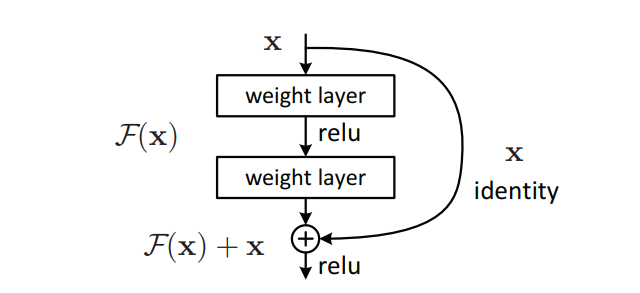
\includegraphics[width=1\linewidth]{Residual-Block}
 		\caption{He és tsai. által javasolt reziduális blokk felépítése.
 			Forrás:\cite{resnet}}
        \label{fig:resblock}
 	\end{figure}
  
    Az eltűnő/explodálódó gradiens problémájának megoldására bevezették a Reziduális/Maradék blokkokat. A hálózatban úgynevezett kihagyásos kapcsolatok jönnek létre. A kihagyásos kapcsolat egy réteg aktivációit úgy kapcsolja össze a további rétegekkel, hogy közben néhány réteget kihagy. Ez egy reziduális blokkot képez. A reziduális hálózatok ezen reziduális blokkok egymásra halmozásával jönnek létre. Az ilyen típusú kihagyásos kapcsolatok hozzáadásának előnye, hogy ha bármelyik réteg károsítja az architektúra teljesítményét, akkor azt a regularizáció kihagyja. Ez tehát egy nagyon mély neurális hálózat tanítását eredményezi az eltűnő/robbanó gradiens okozta problémák nélkül. 

    \subsection{U-Net}

    Ebben a szekcióban Ronneberger és tsai. \cite{unet} munkája alapján bemutatjuk az U-Net architektúrát, amelyet a saját megvalósításunkban a szegmentációs maszk elkészítésére, optimalizálására használunk fel. 

    A konvolúciós hálózatok tipikus felhasználási területe az osztályozási feladatok, ahol
a kép kimenete egyetlen osztálycímke. Azonban számos vizuális feladatban,
különösen az orvosbiológiai képfeldolgozásban, a kívánt kimeneti eredménynek tartalmaznia kell
lokalizációt, azaz minden egyes képponthoz osztálycímkét kell rendelni. Továbbá,
több ezer tanító kép általában elérhetetlen az orvosbiológiai feladatokban.
Ezért Ciresan és tsai. \cite{ciresan} egy csúszóablakos elrendezést alkalmaztak, hogy prediktálják a
az egyes képpontok osztálycímkéjét az adott képpont körüli lokális régió bemenetként történő megadásával.

Ezt az architektúrát úgy módosították és bővítették, hogy
nagyon kevés tanítási képpel működjön, és pontosabb szegmentációkat eredményez.
Az alapötlet a szokásos szűkülő konvolúciós hálózat kiegészítése egymást követő rétegekkel, ahol a pooling operátorokat upsampling operátorok helyettesítik.
Ezért ezek a rétegek növelik a kimenet felbontását. A lokalizáció érdekében a magas
felbontású jellemzőket kombinálják a szűkülő útvonalról származó felskálázott kimenettel. Egy ezt követő konvolúciós réteg ezután megtanulhatja a kimenet precízebb összeállítását ezen információk alapján.

A felfelé mintavételezés
rész nagyszámú funkciócsatornával is rendelkezik, ami lehetővé teszi a hálózat számára, hogy
a kontextusinformációkat továbbítsa a magasabb felbontású rétegek felé. Ennek következtében,
az expanziós útvonal többé-kevésbé szimmetrikus az összehúzódási útvonalhoz képest, és
u alakú architektúrát eredményez.

\subsubsection{Architektúra}

A hálózat felépítését a(z) \ref{fig:unet}. ábra szemlélteti. A rendszer egy szűkülő
(bal oldal) és egy bővülő útvonalból (jobb oldal) áll. Az összehúzódó útvonal
a konvolúciós hálózatok tipikus architektúráját követi. 
Ez a következő lépések ismételt meghívásából áll:
    két 3x3-as konvolúció, melyeket egy-egy ReLU és egy 2x2 max pooling művelet követ. Minden lefelé mintavételezést a jellemzőcsatornák duplázása következik. 

    Az expanzív útvonal minden lépése a jellemzőtérkép felmintavételezéséből áll, amelyet egy 2x2-es konvolúció követ, amely megfelezi a jellemzőcsatornák számát, majd egy konkatenáció a megfelelően levágott jellemzőtérképpel a kontraháló útvonalról, és két 3x3-as konvolúció, amelyet egy-egy ReLU követ. A vágásra a határpixelek elvesztése miatt van szükség
minden egyes konvolúcióban. Az utolsó rétegben egy 1x1-es konvolúciót használnak minden egyes
64 komponensű jellemzővektor a kívánt számú osztályhoz való kötéséhez. Összességében a
hálózat 23 konvolúciós rétegből áll.
    
    \begin{figure}[h]	
 		\centering
 		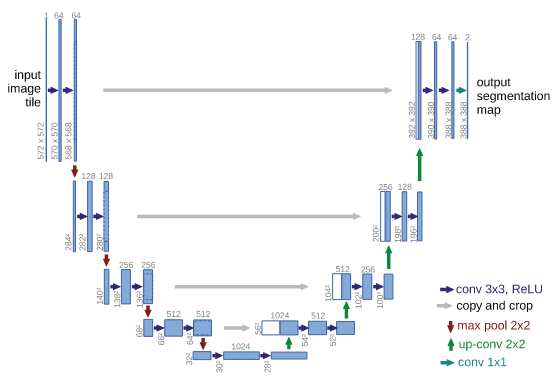
\includegraphics[width=1\linewidth]{unet}
 		\caption{U-Net felépítése
 			Forrás:\cite{unet}}
        \label{fig:unet}
 	\end{figure}
   
	\section{Deep Learning módszerek}
	
	Az előző szakaszok [\nameref{3d}] 2D-ből 3D arc rekonstrukciós módszerei \textit{modelleket} használnak az előzetes tudás megtestesítésére \cite{survey}: a statisztikai modellillesztési módszerek tartalmaznak egy geometriai (és általában textúra) modellt, a fotometriai módszerek pedig a
	az arc fényvisszaverő képességét. 
	
	
	Ezzel szemben a mély tanulási módszerek
	közvetlenül tanulják meg a 2D kép és a 3D arc közötti leképezést, az előzetes ismeretek felhasználásával a betanított hálózatokban.
	
	
	Több indokból is előnyösebb mély tanulási módszerekkel dolgozni.\cite{3dmm}A modellezési oldalon a nemlineáris, mély reprezentációk használata lehetőséget nyújt arra, hogy felülmúljuk a klasszikus lineáris vagy multi-lineáris modelleket az általánosítás szempontjából, tömörség és specifikusság tekintetében \cite{styner}.
	
	
	A paraméter becslési oldalon ki tudjuk használni a mély hálózatok előnyeit, a gyorsaságot és a robusztusságot, hogy megbízható teljesítményt érjünk el a nem ellenőrzött képeken.
	
	\begin{figure}[h]	
		\centering
		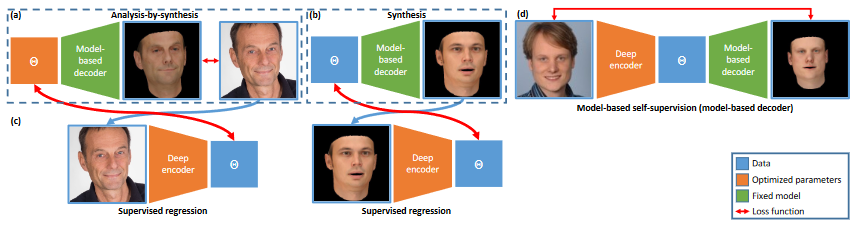
\includegraphics[width=1\linewidth]{deep}
		\caption{A klasszikus analízis-szintézis és a mélytanulási megközelítések közötti kapcsolat. 
			Forrás:\cite{3dmm}}
	\end{figure}
	
	\newpage
	\subsection{Deep Face modellek}
    Ebben az alfejezetben a deep face modellezési módszereket mutatjuk be \cite{3dmm} Egger és tsai. munkája alapján. \\
 
	A hagyományos modellezési technikák célja, hogy
	az arc alakját, arckifejezését és megjelenését $w$ vektorként reprezentálják egy
	alacsony dimenziós látens térben $\mathbb{R}^d$ . A vetítés (illetve rekonstrukció) ebből a latens térből lineáris vagy multi lineáris műveletekkel definiálható, és úgy is felfogható, mint a nagy-dimenziós információ kódolása (ill.
	dekódolása) a $\mathbb{R}^d$ térben.
	
	
	A mélytanulás új eszközt nyújt a 3DMM-ek építéséhez, amely nemlinearitást használ mind a kódolóban és a dekódolóban. Az ilyen \textit{morphable} modellek létrehozása egy jelenleg nagyon aktív kutatási terület.
	Az alak és textúra modellezésre gyakran használt lineáris modellt felhasználva láthatjuk a mélytanulással és a hagyományos módszerekkel tanult kódoló és dekódoló közötti kapcsolatot.
	
	
	A mély tanulás kontextusában egy ilyen lineáris modell
	az alábbi egyenletben formalizálva pontosan megfelel egy teljesen összekapcsolt rétegnek egy
	neurális hálózatban.
	
	\begin{mdframed}
	\begin{equation}
		c(w) = \bar{c} + Ew 
	\end{equation}
		  ahol, $\bar{c}$ a tanítási adatokra számított átlag, $E \in \mathbb{R}^{3n*d}$ egy olyan mátrix, amely tartalmazza a $d$ legdominánsabb sajátvektorjait \\
		  a formakülönbségekre $c_i - \bar{c_i}$ számított kovarianciamátrixban és
		$w$ az alacsony dimenziós alakparaméter-vektor.
	\end{mdframed}
	
	Lényegében, a $w$ paramétervektora bemeneti jellemzők szerepét játssza, az $e_j$ főkomponensek pedig a súlyokét és az átlag $\bar{c}$ a torzítás.
	Ez úgy is felfogható, mint a dekódolás a latens paramétertérből a $c$ adattérbe. Vetítés a modellre
	hasonlóképpen tekinthető egy teljesen összekapcsolt réteggel történő kódolásnak,
	ahol a bemeneti jellemzők az adatok, a súlyok pedig a transzponált főkomponens mátrix sorai, az eltérések pedig adottak $-e^{T}_{j}\bar{c}$ által.
	
	
	 Az analógia lezárásaként a PCA (Principal Component Analysis) a kódoló és a dekódoló egyetlen rejtett réteggel rendelkező lineáris autokódolóvá történő kombinálásával végezhető el.
	Egy ilyen autokódoló $d$ neuronokkal a
	rejtett rétegben egy olyan látens teret fog megtanulni, amelynek kiterjedése megegyezik a $d$
	dimenziós PCA-val, bár az ortogonalitás garanciája nélkül.
	Ez megfelelő veszteségfüggvényekkel biztosítható.
	
	\subsection{Deep Face rekonstrukció}
	
	 A következőkben a mély neurális hálózatokon alapuló sűrű monokuláris arcrekonstrukció megközelítéseket tárgyaljuk. Megbeszéljük
	a felhasznált képzési adatokkal szemben támasztott követelményeket, valamint a különböző képzési
	stratégiákat. 
	
	
	Nézzük meg először közelebbről a rekonstrukciós problémát. Blanz és Vetter \cite{blanzvetter} egy optimalizációs megközelítésen alapuló parametrikus modell illesztésével, azaz a gradiens süllyedéssel kezeli a monokuláris arc rekonstrukcióját. 
	
	
	 A mélytanulási megközelítések hasonló optimalizálási stratégiát követnek, de az optimalizálási probléma 
	tesztelés idején történő megoldása helyett, például egy paraméterregresszort tanítanak be egy nagyméretű képadathalmaz alapján. A regresszor úgy értelmezhető, mint egy kódoló hálózat, amely egy 2D-s képet
	bemenetként fogad és az alacsony dimenziós arcreprezentációt adja ki. 
	
	
	A
	kódolók kombinálhatók klasszikus arcmodelleken alapuló dekódolókkal,
	hogy végponttól-végpontig tartó kódoló-dekódoló architektúrákat hozzanak létre.
	Ez a módszertan széles körben elterjedt és lehetővé teszi a klasszikus
	modellalapú és mélytanulási megközelítések ötvözését.
	
	\subsubsection{Felügyelt rekonstrukció}
	Felügyelt regressziós megközelítések
	párosított tanítási adatok segítségével, azaz egy monokuláris  képgyűjtemény
	és a megfelelő 3DMM paraméterei segítségével tanulnak.
	
	
	Az egyik alapvető kérdés itt az, hogy hogyan lehet hatékonyan megszerezni az adatot egy ilyen felügyelt tanulási feladathoz. A következőkben
	kategorizáljuk a megközelítéseket a
	tanítási adatok alapján. \\
	
	
	Az egyik lehetőség az lenne, hogy a felhasználók határozzák meg az adatot. Míg ez egy népszerű stratégia, amelyet gyakran alkalmaznak rekonstrukciós problémáknál \cite{saragih}, 
	a sűrű geometria, a megjelenés és a helyszín megvilágítás pontos meghatározása szinte megoldhatatlan.
	
	
	Hasonló megközelítést alkalmaztak például Olszewski \cite{olszewski} munkájában,ahol három professzionális animátor kézzel készítette el a \textit{blendshape} animációt egy videokliphez illesztve. A sűrű rekonstrukciós feladatokhoz egyes megközelítéseket ellenőrzött, több nézetből készült felvételek alapján tanítanak be.
	
	
	Így megkapható az adat egy több nézetből történő rekonstrukciós megközelítéssel, amelyet egy 3DMM illesztése követ. Ezáltal  megkapjuk a 3D adatot. Általában az alapadatok nagyon jó minőségűek,
	de a monokulárisan rögzített képek eloszlása nem
	egyezik meg a kontrollálatlan adatokkal, ami általánosítási problémákhoz vezethet
	a tesztelés idejében.\\
	
	
	Anh Tuan Tran megközelítése monokuláris rekonstrukciót végez ugyanarról a személyről készült több képre, és kiszámít egy konszolidált arcazonosságot a 3DMM paraméterek egyszerű átlagolása alapján. \\
	
	
	Jelenleg a kutatóközösségben számos megközelítés szintetikus tanítási adatokat használ tanításhoz, mivel könnyen beszerezhető és tökéletes annotációkkal rendelkeznek. 
	
	
	Adott egy 3DMM arc, véletlenszerű identifikációk és kifejezések mintavételezhetők a paramétertérben. 
	Majd
	a modelleket véletlenszerű megvilágítási körülmények között és különböző nézőpontokból lehet renderelni a monokuláris képek létrehozásához. 
	
	
	A háttértámogatást gyakran alkalmazzák úgy, hogy a generált arcokat a valós világ sokféle hátterére renderelik. Mivel az összes paramétert ellenőrzik, ezért azok kifejezetten ismertek, és alapigazságként használhatók.
	
	
	Míg könnyen hozzájuthatunk a szintetikus képzési adatokhoz, gyakran van egy nagy tartományi rés
	a szintetikus és a valós világ képei között, ami súlyosan befolyásolja a
	a valós képekre való általánosítást. Például a hajat, az arcszőrzetet, a felsőtestet,
	vagy a száj belsejét gyakran egyáltalán nem modellezik. Az egyik lehetőség,
	a jövőben olyan modelleket használni, amelyek tartalmazzák ezeket, hogy ellensúlyozzuk ezt a problémát. 
	
	
	A valós és a szintetikus képzési adatok előnyeinek kihasználása érdekében számos jelenlegi megközelítést e két terület adatainak keverékével tanítanak. A remény itt az, hogy a megközelítés megtanulja kezelni a valós világi
	képeket, miközben a szintetikus tréning adatok tökéletes alapigazsága
	segítségével stabilizálható a tanulás.\\


	Ennek egy érdekes változata
	a tanítás önfelügyelt \textit{bootstrappelése}. A további megközelítéseket, amelyek tanítása nem igényel
	alapigazságadatokat a következő fejezetben vizsgáljuk meg.
	
	\subsubsection{Önfelügyelt rekonstrukció}
	A konvolúciós neurális hálózatok felügyelt tanítása annotált adathalmazt igényel. A legtöbb
	eddig tárgyalt módszer ilyen - szintetikus vagy valós - adathalmazokat használ.
	
	\cite{3dmm}
	A közelmúltban egyes megközelítések önfelügyeletet alkalmazó
	tanulást használtak, azaz 3D címkék nélküli, valós képi adathalmazokon történő tanítást.
	Ezt az analízis-szintézis és a mélytanulási technikák kombinációja tette lehetővé.
	
	
	Tewari és tsai. \cite{tewari} egy modell-alapú kódoló-dekódoló architektúrát mutatott be, amely a
	a betanítható dekódert egy fix dekóderrel helyettesíti. Ez a dekóder a 3DMM paramétereket (látens kód)
	mint bemenet, amelyet a kódoló jelez, a 3DMM segítségével 3D-rekonstrukcióvá alakítja.
	Továbbá szintetikus képet készít a rekonstrukcióról egy differenciálható renderelő segítségével.
	A rendereléshez szükséges külső paramétereket szintén a kódoló jelzi előre. 
	
	
	Az alkalmazott veszteségfüggvény nagyon hasonlít az analízis-szintézisben használthoz \cite{3dmm}, ami fotometriai igazítást és statisztikai szabályozást foglal magába. Egy ilyen technikára úgy is gondolhatunk, mint egy közös
	\textit{analysis-by-synthesis} optimalizálási probléma egy nagyméretű tanulási
	adathalmazon, egyetlen kép helyett. Ez lehetővé teszi a paraméterregresszor képzését 3D felügyelet nélkül.
	
	\newpage
	\section{Megvalósítás}
	
	Ebben a fejezetben a projektünk redszertervét, gépi tanulási pipeline-ját, valamint kulcsfontosságú metódusait mutatjuk be részletesen.
	
	\subsection{Felhő alapú architektúra}
	
	\begin{figure}[h]	
		\centering
		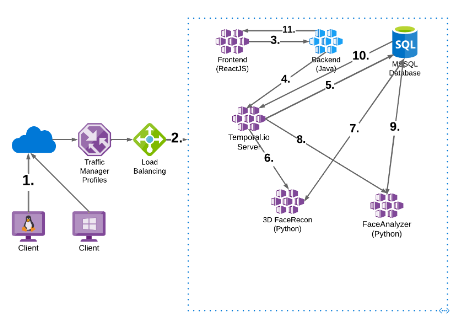
\includegraphics[width=1\linewidth]{sysplan}
		\caption{ A rendszer felépítése}
	   \label{fig:sysplan}
    \end{figure}

	Ahogy korábban is említettük, a kitüzőtt céljaink között van, hogy a
	3D arc rekonstrukció és az arc analízis elérhető legyen felhőn keresztül.
	Továbbiakban megvizsgáljuk a rendszer felépítését illetve mükődését a
	fenti ábra segítségével. A(z) \ref{fig:sysplan}. ábrán látható, hogy 6 különböző szolgáltatást
	Minikube lokális klaszteren üzemeltetünk.

    \newpage
	\begin{mdframed}
		A minikube egy helyi Kubernetes, amellyel gyorsan tudunk létrehozni
		egy lokális klasztert, amely megkönnyíti a Kuberneteshez való tanulást
		́es fejlesztést
	\end{mdframed}

	A 6 különböző szolgáltatás az alábbiak:
	\begin{itemize}
		\item Frontend
		\item Backend
		\item Temporal.io szerver
		\item 3D arcrekonstrukciós modul
		\item Arcanalízis modul
		\item Adatbázis
	\end{itemize}

	A Temporal.io egy olyan technológia amely segítségével gyorsan és
	egyszerűen tudunk workflow-t implementálni. Ehhez szükséges a szerver,
	mert ott bonyolódik le egy workflow sikeres elvégzése, vagy hiba esetén
	biztosít egy dashboard-t amivel megtudjuk vizsgálni a hiba okát. Illetve,a
	workflow-ban implementáltuk a SAGA programozási mintát, amely kezeli
	hibák esetén az adatbázissal kapcsolatos műveleteket. Ezzel is robosztusabbá
	teszi a rendszert.
	
	Ha megnézzük a fenti ábrát, láthatjuk hogy, a workflow belépési pontja a HTTP kérés, aminek payload-ja, a kép egy célszemélyről, és amint a
	frontend-től megkapja a kérést a backend, az elindítja a workflow-t. A következő lépés hogy, a workflow metódusai egymás után meghívódnak.
	Végül a felhasználó visszakapja a rekonstruált képet, illetve a képen lévő személy akkori érzelmi állapotát és életkorát. Az arcrekonstrukciós és arc
	analízis moduljainkat Python nyelven implementáltuk, mivel mesterséges intelligenciával dolgozunk, a különböző nagymennyiségű Python könyvtár
	elérhetősége nagy mértékben megsegítette munkánkat.
	
	
	\newpage
    \subsection{Arcrekonstrukció}

    Ebben a fejezetben az arcrekonstrukciós hálózatunk felépitését és müködését vizsgáljuk meg és a hozzákapcsolodó technológiákat.

    \subsubsection{Tanítási adathalmazok}
	A rekonstrukciós modellünk a nyilvánosan elérhető CELEBA adathalmazból tanul \cite{celeba}. A $CelebFaces Attributes Dataset$ (CelebA) egy nagyméretű arcattribútum adatkészlet, amely több mint 200 000 híresség képét tartalmazza, mindegyikhez 40 attribútum annotáció tartozik. Az adatállomány képei nagy pózvariációkat és háttérzavarokat fednek le. A CelebA nagy változatossággal, nagy mennyiségben és gazdag annotációkkal rendelkezik, többek között az alábbiakkal:

    \begin{itemize}
        \item 10 177 különböző személyazonosság
        \item 202 599 számú arckép
        \item 5 jellegzetes arcpont, képenként 40 bináris attribútum annotációja
    \end{itemize}

    \begin{table}[h]
        \begin{tabular}{lll}
        Adathalmaz    & \begin{tabular}[c]{@{}l@{}}Darabszám\end{tabular}\\
        tanuló    & 162770                                                           \\
        validációs & 19962                                                           \\
        teszt       & 19868                    
        \end{tabular}
    \end{table}

	\subsubsection{Adatok előkészítése}

   A valósághű 3D arcrekonstrukció elérése érdekében fontos, hogy az adatokat előkészítsük még a tanítási folyamat előtt. Ez a lépés a munkánkban az arc jellegzetes pontjainak detektálását, majd a pontok \textit{.csv} fáljokba való kiírását jelenti. Yao Feng és tsai. \cite{deca} megközelítését követve \cite{bulat}Bulat és tsai. FAN modelljét használjuk a 68 db 2D-s jellegzetes pont (landmark) detektálásához. A FAN egy arcpontok lokalizálására szolgáló reziduális hálózaton alapuló architektúra, amelyet  egy nagy, de szintetikusan kibővített 2D-s arcpont-adathalmazon tanítottak. Ezután 5 adathalmazon, nagyjából 230 000 képpel értékelték ki a hálózatot és átlagosan 68,36\%-os pontosságot értek el.

   \subsubsection{Adatok előkészítésének megvalósítása}

   A \textit{list\_eval\_partition.csv} megadja, hogy az adott kép melyik adathalmazhoz tartozik.
   A három adathalmaz a tanító, a tesztelési és a validációs halmazok. A FAN modellt felhasználva detektáljuk képenként a 68 db arcpontot, majd azok mentésre kerülnek a kép partíciójának megfelelő .csv fájlba. A .csv fájlok a \textit{train\_landmarks.csv}, \textit{test\_landmarks.csv} és a \textit{val\_landmarks.csv}.
				
    \subsubsection{FAN modell}
    
     face-alignment egy Python-csomag, amely egy olyan eszközkészletet biztosít, amely az arc tájékozódási pontjainak felismerésére, a fej pózának becslésére és az arc igazítására szolgál. 
     Mély tanulási modelleken alapul, és az arcképek előfeldolgozására használható olyan feladatok elvégzése előtt, mint az arcfelismerés vagy az érzelemérzékelés.
    
    A csomag több modulból áll, amelyek mindegyike az arcelemzéssel kapcsolatos speciális feladatot lát el. Az alábbiakban röviden áttekintjük az egyes modulokat:

    \begin{itemize}
        \item \textbf{észlelés}: 
        
        Ez a modul SSD (Single Shot Detector) architektúrán alapul és előre betanított modelleket használó arcfelismerő funkciókat biztosít. Az arcdetektor betanítható az arcok felismerésére különböző beállítások mellett, például gyenge fényviszonyok, eltakart arcok vagy profilnézet esetén.

        \item \textbf{igazítás}: 
        
        Ez a modul funkciókat biztosít az arc tájékozódási pontjainak felismeréséhez és az arcok igazításához.
		A tájékozódási pont detektor egy mély konvolúciós neurális hálózatot (CNN) használ az arc kulcsfontosságú pontjainak, például a szemeknek, az orrnak és a szájnak a helyzetének a felismerésére. 
		Az arcigazítási funkció ezután a tájékozódási pontok pozícióit használja fel az arckép geometriai transzformációjának elvégzéséhez.


        \item \textbf{póz}: 
        
        Ez a modul funkciókat biztosít az arc fejpózának becslésére, ami a fej kamerához viszonyított orientációját jelenti. A pózbecslő egy CNN-t használ a fej gördülési és dőlési szögének becslésére.
        \item \textbf{segédeszközök}: Ez a modul egy sor segédfunkciót biztosít a képfeldolgozáshoz, mint például a méretváltoztatás, a képkivágás és a színnormalizálás.

    \end{itemize}

   
    \subsubsection{U-Net tanítási adatok generálása}
    A szegmentáló hálózat súlyainak durva inicializálása érdekében a hálózatot elő kell tanítanunk. A hálózat (U-Net) előtanításához adatokat kell generálnunk. A szegmentációs maszkok elkészítéséhez a $face-toolbox-keras$ \url{https://github.com/shaoanlu/face_toolbox_keras} könyvtárat használjuk azon belül is a BiSeNet modellen alapuló modult \url{https://github.com/zllrunning/face-parsing.PyTorch}. A könyvtár által generált maszk azonban még nem megfelelő számunkra mivel nem csak az arcot veszi figyelembe, hanem a különböző kitakaró tényezőket is. Számunkra a maszkon csak az számit hogy, az adott pixel része-e az arcnak. Ebből adódóan a generált maszkot át kell alakítanunk olyan formában, hogy a maszkon 1-es számmal jelölje azokat a pixeleket, amelyek az arc részei, valamint 0-val, ha az arc nem tartalmazza az adott képpontot. Eredményként egy fekete-fehér maszkot kapunk, amelyen a fehér szín jelöli az arcmaszkot. Ezt a folyamatot az egész tanítási adathalmazon végrehajtjuk. 
    Az előtanított arcrekonstrukciós modellünkkel 3D-s renderelt képeket gyártunk, valamint a bemeneti képeket is felhasználjuk a szegmentációs hálózat előtanításához.
    

    \subsubsection{Arcrekonstrukciós hálózat előtanítása}
    
    \subsubsection{Differenciálható renderelő}

    Ebben a fejezetben Kato et al. \cite{diffrenderer} kutatása alapján bemutatjuk a differenciálható renderelő alapelvét.

    A legtöbb 3D becslési módszer a
felügyelt tanítási rendszerekre és költséges címkézésekre támaszkodnak, ami
a 3D megfigyelések összes paraméterének összegyűjtését jelentősen megnehezíti.
Az egyik
megközelítések egyike a grafikus renderelési folyamatok integrálása
a neurális hálózattal működő rendszerekbe. Ez lehetővé teszi az átalakítást és
a 3D becslések beépítését a 2D képi szintű bizonyítékokba.

A számítógépes grafikában a renderelés a geometria, a jelenet fényei és a kamera tulajdonságai alapján történő 3D-s jelenetek képének előállítását jelenti.

A differenciálható renderelés (DR) olyan technikák családját alkotja, amelyek a renderelési folyamat hasznos gradienseinek kinyerésével végponttól végpontig tartó optimalizálás céljából integrációt valósítanak meg. A renderelés differenciálásával a DR áthidalja a szakadékot.
a 2D és a 3D feldolgozási módszerek között, lehetővé téve a neurális hálózatok számára, hogy 2D-s vetületeken dolgozva optimalizálják a 3D-s entitásokat. Amint a(z) \ref{fig:diffrenderer}. ábrán látható, a 3D jelenet paramétereinek optimalizálása a gradiensek visszaterjedésével érhető el a renderelési kimenethez képest. 

Az általános 3D önfelügyeleti modell a renderelő réteg integrálásával a megjósolt jelenetparaméterekhez és a veszteség alkalmazásával a renderelt és a bemeneti kép különböző módokon történő összehasonlításával történik.

    \begin{figure}[h]	
		\centering
		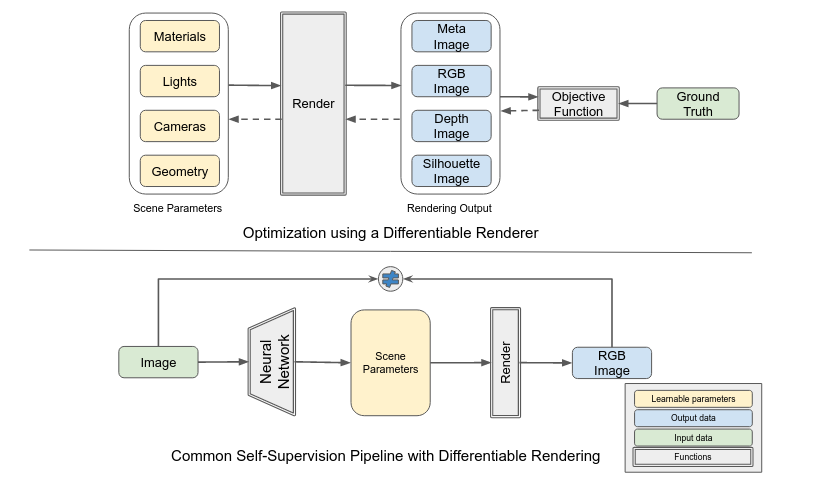
\includegraphics[width=1\linewidth]{diffrenderer}
		\caption{Általános önfelügyeleti modell differenciálható rendereléssel.\\
                Forrás: \cite{diffrenderer}}
        \label{fig:diffrenderer}
	\end{figure}
 \newpage

\subsubsection{Sztenderd raszterizáló megvalósítása}
A sztenderd raszterizáló a rasterizer.py fájlban van implementálva.
 Ez a raszterizáló egy 3D-s archálót kap, amelyet csúcsok és lapok halmaza reprezentál, és egy 2D-s képsíkra vetíti, hogy az arc textúrázott képét létrehozza.
 A raszterizáló a következő lépések szerint működik:
 \begin{enumerate}
     \item \textbf{Perspektív vetítési mátrix létrehozása}:
     A perspektív vetítési mátrix egy 4x4-es mátrix, amely a 3D koordinátákat 2D képkoordinátákra képezi le. 
	A mátrix kiszámítása a kamera kalibrációs paramétereinek felhasználásával történik, amelyek közé tartozik a kamera belső mátrixa, külső mátrixa és a képméret. 
Az belső mátrix a kamera belső paramétereit, például a fókusztávolságot, a főpontot, 
és a dőlést tartalmazza, míg az külső mátrix a kamera helyzetét és tájolását a világkoordináta-rendszerben.
     \item \textbf{A vetítési mátrix alkalmazása a a csúcsokra}:
     
     A 3D archáló csúcsait homogén koordinátákká alakítjuk át egy negyedik dimenzió hozzáadásával, amelynek értéke 1. 
	Ezután a perspektivikus vetítési mátrixot alkalmazzuk a csúcsokra, hogy megkapjuk a megfelelő 2D-s képkoordinátákat. 
	A 2D képkoordinátákat úgy kapjuk meg, hogy az x és y koordinátákat elosztjuk a homogén w-koordinátával.
 
     \item \textbf{A háromszögek határoló dobozainak kiszámítása}:
     
     A háromszögek határoló dobozait az archálóban 2D-s képkoordinátákban kell kiszámítani.
	A határoló dobozokat a háromszög csúcsainak minimális és maximális x és y koordinátái határozzák meg.
 
     \item \textbf{A háromszögek raszterizálása}:
     
     A raszterizáló az archáló minden egyes háromszögéhez kiszámít egy maszkot, amely jelzi, hogy a 2D-s kép mely pixelei tartoznak a háromszöghöz. 
A maszk kiszámítása a háromszög csúcsainak baricentrikus koordinátáinak interpolációjával történik a háromszög határoló dobozán.
	A baricentrikus koordinátákat a csúcsok súlyaként határozzuk meg, amelyek összege egy, és a háromszög textúrakoordinátáinak és csúcsnormálisainak interpolálásához használjuk.
 
     \item \textbf{Textúra leképezése}:
     
     A raszterizáló a raszterizált háromszögekhez a textúra hozzárendelésével  hozza létre a végső képet. 
A textúratérképezés során a háromszögben lévő minden egyes pixel textúrakoordinátáit a baricentrikus koordináták és a háromszög csúcsainak textúrakoordinátái alapján számítja ki.
	Ezután a textúrakoordinátákat a megfelelő helyen a textúrakép mintavételezéséhez használjuk, és a mintavételezett texel színértékét rendeljük a pixelhez.
 
     \item \textbf{Alfa keverés}:
     
     A raszterizáló az átlátszóság kezelése érdekében alfa keverést alkalmaz a raszterizált háromszögekre. 
	A háromszögben lévő egyes pixelek alfa-értékét a baricentrikus koordináták és a háromszög csúcsainak alfa-értékei alapján számítja ki. 
	Ezután az alfa-értékek segítségével a pixel színértéke a háttérszínnel keveredik.
 
 \end{enumerate}
 
 Összességében a sztenderd raszterizáló a 3D archáló renderelésének robusztus és hatékony megvalósítását biztosítja.
 A raszterizáló testreszabható és bővíthető, hogy különböző textúra leképezési és keverési technikákat, valamint különböző renderelési lehetőségeket, például világítást és árnyékolást alkalmazzon.

\subsubsection{SRenderY renderelési módszer és megvalósítása}


 A differenciálható renderelés egy olyan renderelési módszer, amely a kamera paraméterei, a csúcsok pozíciói és a textúra leképezések alapján egy 3D-s arc háló 2D-s képét generálja. A metódus implementációját a renderer.py SRenderY osztálya tartalmazza. 

 Az SRenderY módszer mükődése:

 \begin{enumerate}
 
    \item Egy üres (H, W, 3) méretű képpuffer inicializálása, ahol H és W a kimeneti kép magassága és szélessége pixelben, 3 pedig a színcsatornák száma (piros, zöld és kék).

    \item A 3D archáló minden egyes háromszögéhez kiszámítja a 2D-s vetületét a képsíkra a kamera paraméterei alapján. Ez a perspektivikus vetítési egyenlet segítségével történik, 
 amely a világkoordinátarendszer 3D pontjait a képsík 2D pontjaivá alakítja át.

    \item A kivetített háromszög határoló dobozán belüli minden egyes pixel esetében ellenőrzésre kerül a baricentrikus koordináta módszerrel, hogy a pixel a háromszögben van-e. 
Ennek során kiszámítja a pixel baricentrikus koordinátáit a háromszög csúcsaihoz képest, és ellenőrizzük, hogy ezek mindegyike pozitív-e.
 
    \item Ha a képpont a háromszög belsejében van, akkor az inverz perspektivikus vetítési egyenlet segítségével kiszámítja a megfelelő 3D pozícióját az arc hálóján.

    \item A pixel textúrakoordinátáinak interpolálása a háromszög csúcsainak textúrakoordinátáiból a baricentrikus koordináták segítségével.

    \item Az interpolált textúrakoordináták felhasználása a megfelelő helyen lévő textúratérkép színértékének mintavételezéséhez.

    \item A színérték megszorzása a megvilágítási értékkel, amelyet a pixel felszíni normálisa és a fény iránya közötti skalárszorzataként számítunk ki.

    \item A színérték felhalmozása a képponthoz a képpufferben.

    \item A 2-8. lépés megismétlése a 3D archáló összes háromszögére.

    \item Visszaadja a végső képpuffer képét kimenetként.
    
 \end{enumerate}

 Összességében az SRenderY módszer egy sztenderd raszterizáció-alapú renderelési algoritmus, amely figyelembe veszi a perspektivikus vetítést,
textúratérképezést és a megvilágítást. A DECA keretrendszerre építve 3D-s archáló 2D-s képének létrehozására használjuk.

\subsubsection{Megvilágítás hozzáadása}
A renderer.py add\_SHlight metódusa egy olyan módszer, amely gömbharmonikus (SH) megvilágítást ad hozzá egy 3D-s archáló 2D-s képéhez.

Az add\_SHlight (\textit{Spherical Harmonics}) módszer működése:

\begin{enumerate}
    \item Egy üres (H, W, 3) méretű képpuffer inicializálása, ahol H és W a bemeneti kép magassága és szélessége pixelben, 3 pedig a színcsatornák száma (piros, zöld és kék).

    \item Kiszámítja a világítás gömbharmonikus (SH) együtthatóit az SH-projekciós módszerrel, amely a világítási függvény ortonormális SH-alapfüggvények halmazára való vetítését jelenti.

    \item A bemeneti kép minden egyes pixelére kiszámolja az archáló megfelelő 3D pontjának felületi normálisát. Ez elvégezhető az arc geometriájának a 2D képkoordinátákhoz viszonyított részleges deriváltjainak segítségével.

    \item Értékelje ki az SH megvilágítási függvényt a képpont felületi normálisán a 2. lépés SH együtthatóinak felhasználásával. Ehhez ki kell számítani az SH alapfüggvények és a felületi normális vektor közötti skalárszorzatot.

    \item Megszorozza a bemeneti kép pixelének színértékét a 4. lépésben kiszámított SH megvilágítási értékkel.

    \item A kapott színértéket a [0, 255] tartományba kell szorítani, hogy a 8 bites színértékek érvényes tartományába essen.

    \item A kimeneti képpuffer kép pixelének színét a rögzített színértékre állítja.

    \item Megismétli a 3-7. lépést a bemeneti kép összes pixelére.

    \item Visszaadja a végső képpuffer képét kimenetként.

    
\end{enumerate}

Összességében az add\_SHlight módszer egy meglehetősen szabványos módszer SH megvilágítás hozzáadására egy 3D-s arc háló 2D-s képéhez. A világítási függvény SH-együtthatóinak kiszámítását, 
az SH-világítás kiértékelését minden egyes felületi normálisnál, és az egyes pixelek színértékének megszorzását az így kapott világítási értékkel foglalja magában. 
Ezt a módszert a DECA keretrendszer alapján a 3D-s arcok SH megvilágítással ellátott hálóinak valósághű 2D-s képeinek létrehozására használjuk.

\subsubsection{Normáltérkép kiszámítása eltolódási térképből}

A displacement2normal függvény arra szolgál, hogy az elmozdulási térképből kiszámítsa a normáltérképet, amelyre a renderelésnél lesz szükségünk. 
A számítógépes grafikában az elmozdulási térkép egy olyan textúra, amely egy objektum felületének elmozdulását kódolja.
A textúrában lévő elmozdulási értékek jellemzően a felületre merőleges irányban vannak meghatározva, ami azt jelenti, hogy felhasználhatóak a normáltérkép kiszámításához.

A displacement2normal függvény bemenetként egy elmozdulási térképet és a térképen lévő pixelek textúrakoordinátáit veszi fel. 
Az elmozdulási térképet szürkeárnyalatos képnek tekintjük, ahol az értékek a felületre merőleges irányú elmozdulást jelölik.
A textúrakoordináták a textúra képpontjainak 2D koordinátái.

A normáltérkép kiszámításához a függvény először kiszámítja az elmozdulási térkép részleges deriváltjait a textúrakoordinátákhoz képest.
Ezek a parciális deriváltak a felület x és y irányú meredekségét jelentik. A parciális deriváltakat ezután a felület normális vektorának kiszámítására használjuk minden egyes pixelnél.

A normálvektor kiszámításához a függvény először kiszámítja a felület érintővektorát és bitangens vektorát.
Az érintővektort az x irányú parciális derivált és az (1, 0, 0) vektor keresztszorzataként számoljuk ki. 
A bitangens vektor az y irányú parciális derivált és a (0, 1, 0) vektor keresztszorzataként számítandó. 
Végül a normálvektort az érintővektor és a bitangens vektor keresztszorzataként számítjuk ki.

Az így kapott normáltérkép egy 3 csatornás kép, ahol minden egyes pixel egy normálvektort képvisel. 
A normálvektor x, y és z komponenseit a vörös, zöld és kék csatornákban kódoljuk. 
A normálvektort úgy normalizáljuk, hogy egységnyi hosszúságú legyen.

Összességében a displacement2normal függvény lehetővé teszi az elmozdulás-térkép normál-térképpé alakítását, amely egy objektum felületének nagy felbontású részletekkel történő szimulálására használható.

\subsubsection{Tanítás}
    \begin{figure}[h]	
		\centering
		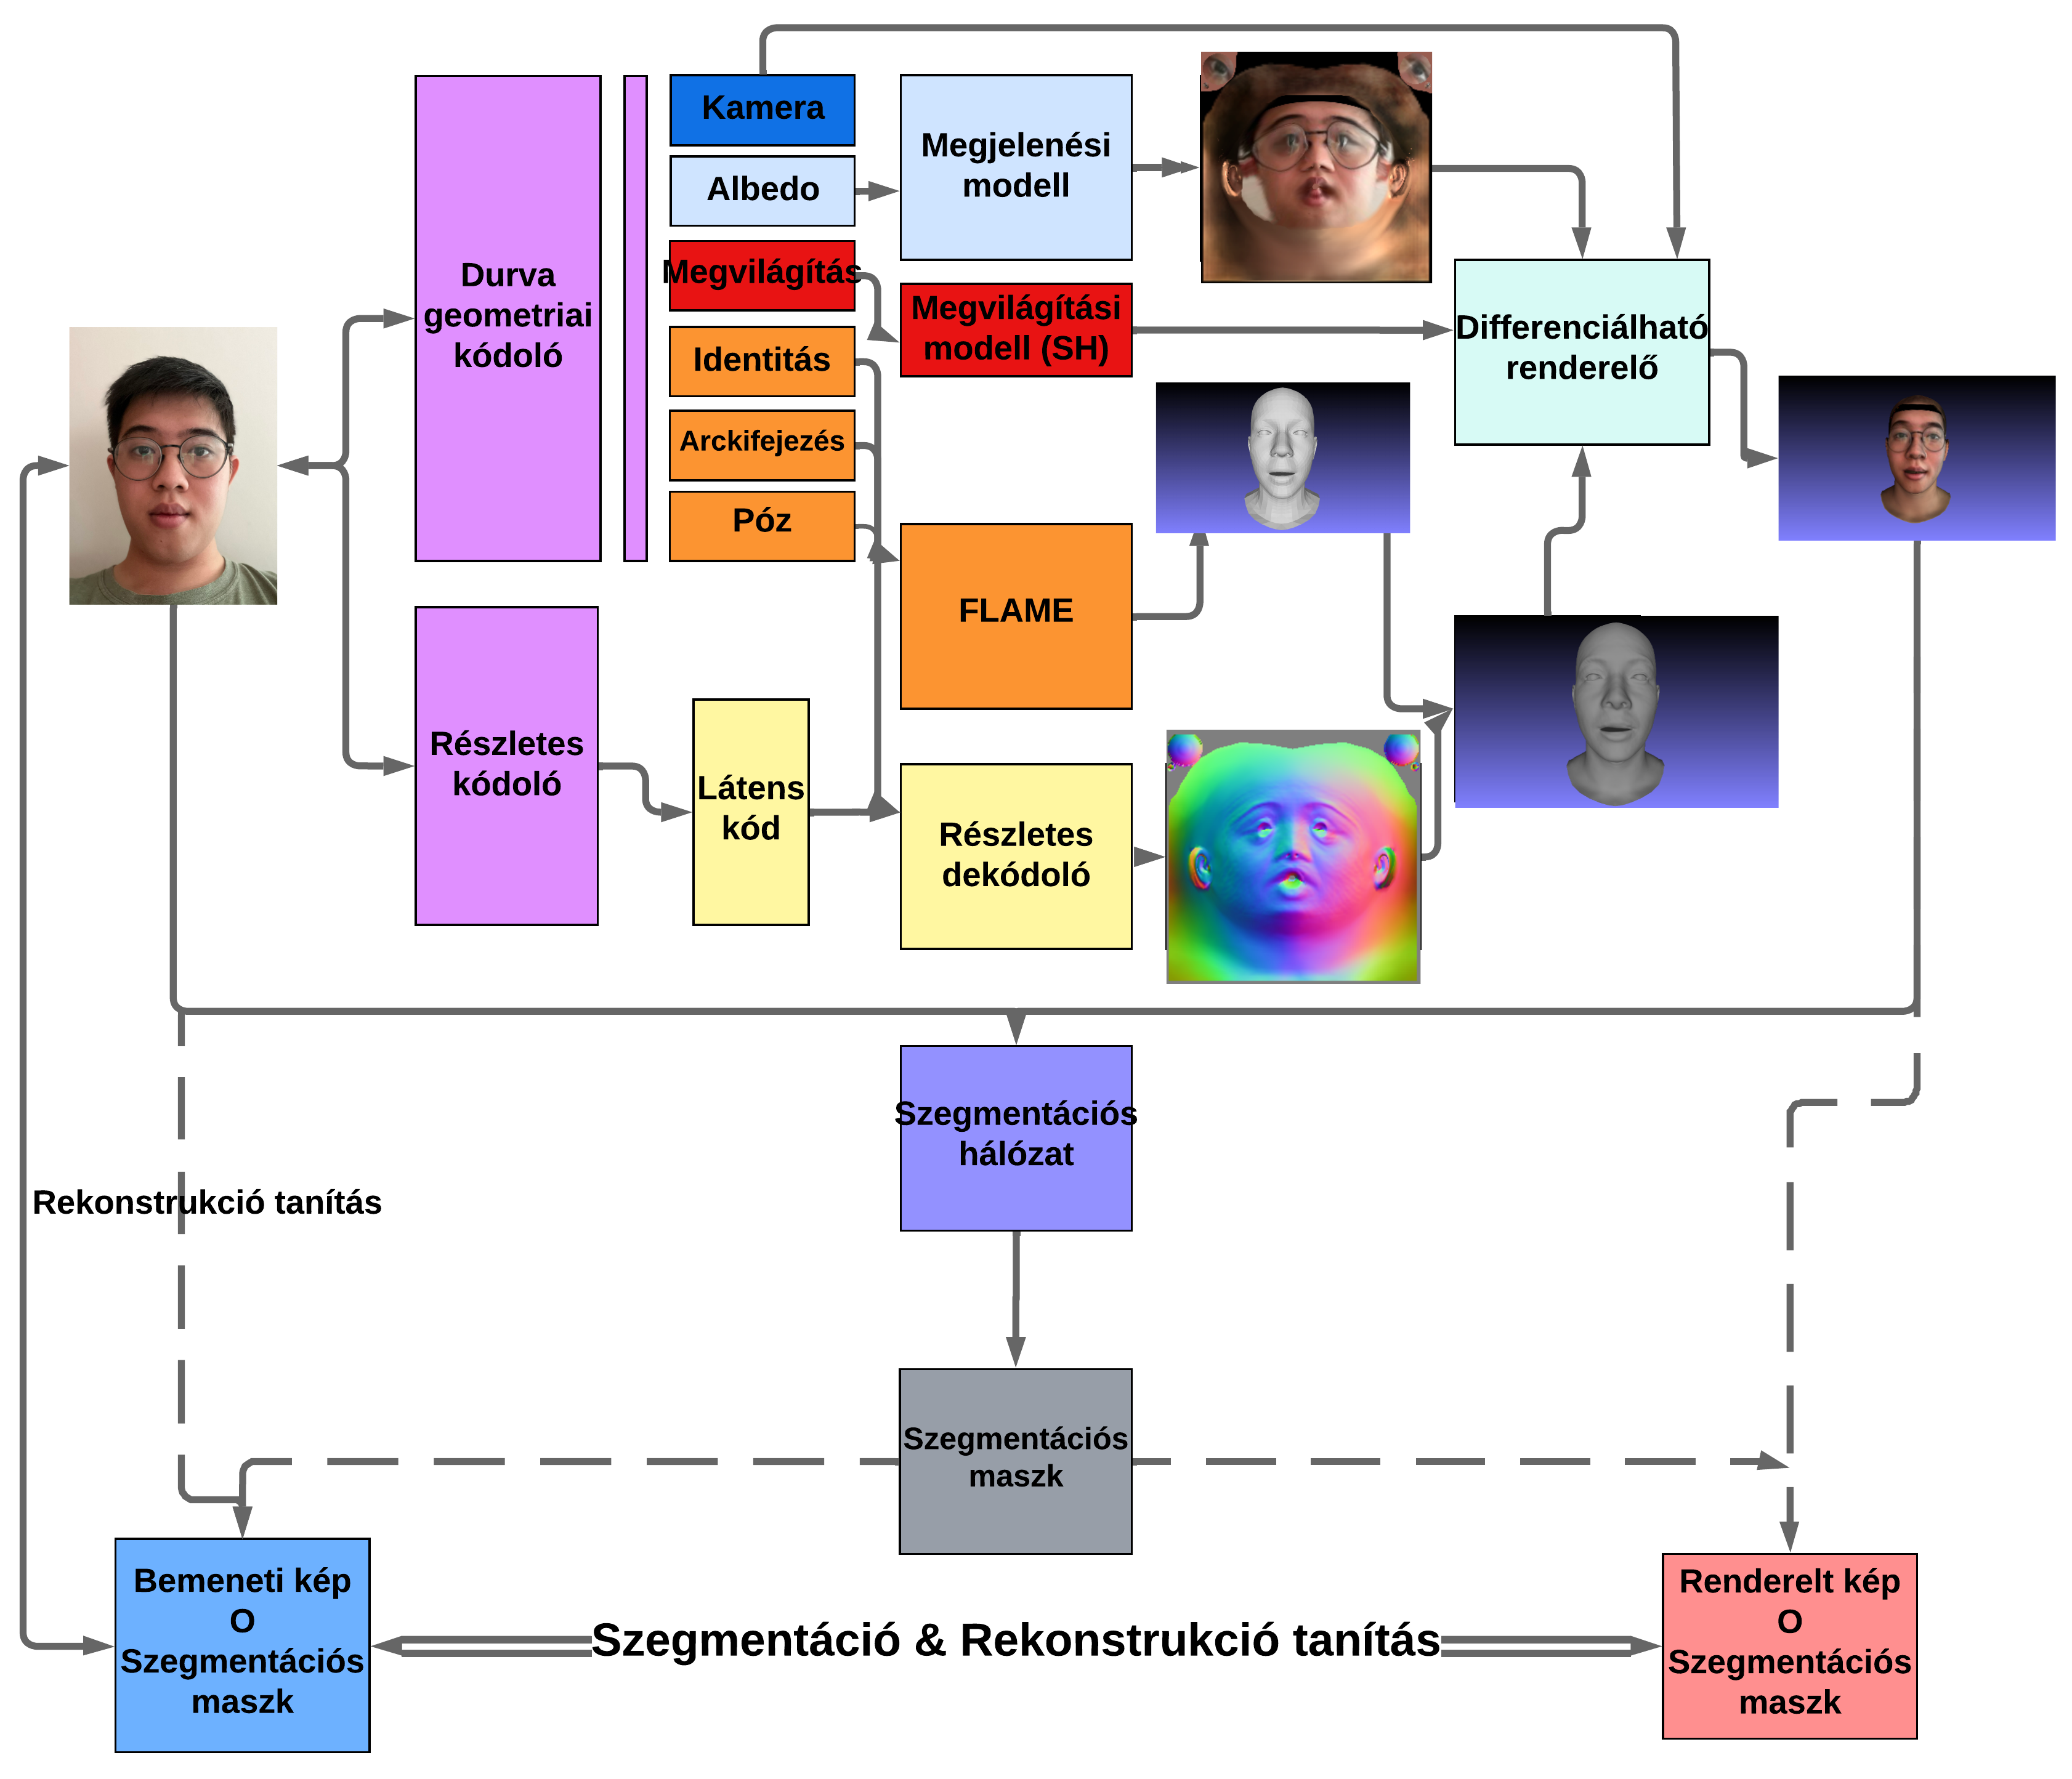
\includegraphics[width=1\linewidth]{pipelinehun}
		\caption{  A rekonstrukciós hálózat tanítási futószalagja.}
        \label{fig:pipeline}
	\end{figure}
 
	Az arcreskonstrukciós modellünket a(z) \ref{fig:pipeline}. ábrán szemléltetjük. A hálózatot PyTorch
	keretrendszerben fejlesztettük.
	A DECA módszerét követve a hálózatunk első lépése egy
	ResNet-50 modulból és egy teljesen összekapcsolt rétegből álló kódoló
	$E_{c}$, amely egy 2D-s kontrollálatlan környezetben készült képet kap bementként, majd visszaadja annak alacsony dimenzós látens kódját.
 
 A látens kód a $FLAME$
	paramétereket (durva geometriát) $\beta$ $\psi$ $\theta$, valamint az albedo együtthatókat
	$\alpha$, kamera $c$, és megvilágítási $l$ paramétereket tartalmazza.
	Az albedó paramétereket megkapja
	bemenetként a megjelenési modell, amely a Basel Face Model (BFM)
	lineáris albedó alterét alakítja át a $FLAME$ UV elrendezésébe,
	hogy kompatibilissé tegye azt $FLAME$-el A megvilágítási paramétereket
	a megvilágítási modell kapja meg bemenetként amely,
	a Spherical Harmonics (SH) alapú.
 
 A durva geometria
	paramétereit felhasználva a $FLAME$ modell egy durva alakzatot készít az
	arcról. 
 
 A DECA által javasolt részletes dekódolóba a 128 db személyspecifikus jellemzőt betáplálva egy UV eltolódási térképet készítünk. A durva alakot és az eltolódási térképet felhasználva egy részletes alakzatot készítünk, amelyet átadva a megvilágítási modellel,
	az albedó térképpel, és a kamera paraméterekkel a differenciálható renderelőnek egy részletes rekonstruált textúrázott 3D-s fejet kapunk kimenetül.

 
	A $FOCUS$ megközelítéséhez hasonlóan,a szegmentáló hálózatunk átveszi
	a bemeneti képet és a hozzá tartozó részletes rekonstruált 3D-s fejet, majd
	megjósolja a bináris maszkot.

     \subsubsection{Arcrekonstrukciós hálózat tanításának megvalósítása}
    Az arcrekonstrukciós modell tanítási folyamata több lépésre osztható:

    \begin{enumerate}
        \item \textbf{Adatbővítés}:
        
        A modell általánosítási képességének javítása érdekében a tanítási adatokra adatbővítést alkalmazunk. Ez magában foglalja a képek véletlenszerű vágását, átméretezését és átfordítását, valamint a FLAME paraméterek véletlenszerű torzítását.
        \item \textbf{Modellarchitektúra}:
        
        Az arcrekonstrukciós modell egy mély neurális hálózat,
       amely egy kódolóból és egy dekódolóból áll. 
        A kódoló a bemeneti paramétereket egy látens térbe képezi le, 
        míg a dekódoló a látens teret képezi vissza a FLAME paraméterekre. 
        A kódoló egy ResNet-50 hálózat, míg a dekódoló egy teljesen összekapcsolt hálózat kihagyásos kapcsolatokkal.
    
    A kódoló és dekódoló függvényeket arra használjuk, hogy egy emberi arc 3D-s hálós modelljét átalakítsunk vagy visszaalakítsunk egy paraméterezett reprezentációból a FLAME modell segítségével.
        
        \item \textbf{Kódoló}:
        A kódoló egy emberi arc 3D-s hálómodelljét veszi fel bemenetként egy numpy tömb formájában, amely a csúcspontok koordinátáit és egy numpy tömböt tartalmaz, amely a csúcspontok színét tartalmazza.
A függvény ezután a FLAME modell segítségével kiszámítja az arc alakját, arckifejezését és pózát leíró paraméterek halmazát.

        \textbf{A kódoló lépései}:
        \begin{enumerate}
            \item \textbf{FLAME model betöltése}:
            
            Az enkódoló függvény először betölti a FLAME modellt egy előre betanított PyTorch ellenőrzőpont fájlból. 
Ez a modell lineáris alak, kifejezés és póz alapfüggvényekből, valamint egy sor tanult nemlineáris korrekciós LBS súlyokból áll.

            \item \textbf{Alak, kifejezés és póz paraméterek kiszámítása}:
            
            A kódolási funkció a FLAME modell segítségével kiszámítja az alak, a kifejezés és a póz paramétereit, amelyek leírják a 3D hálómodellt. 
Ez egy olyan költségfüggvény minimalizálásával történik, amely a bemeneti 3D hálómodell és a FLAME paraméterekből rekonstruált modell közötti különbséget méri. 
A költségfüggvény olyan feltételeket tartalmaz, amelyek büntetik a FLAME-modell alak-, kifejezés- és pózprioritásától való eltéréseket.

            \item \textbf{Paraméteres reprezentáció visszaadása}:

            A kódoló függvény egy szótárat ad vissza, amely tartalmazza a kiszámított alak, kifejezés és póz paramétereit, valamint az LBS súlyokat és egyéb modellparamétereket.

        \end{enumerate}
        

        
        \item \textbf{Dekódoló}:

        A dekódoló függvény bemenetként egy emberi arc paraméterezett reprezentációját veszi át, amely egy alak-, kifejezés- és pózparamétereket tartalmazó szótár formájában jelenik meg, 
valamint az LBS súlyokat és egyéb modellparamétereket. A függvény ezután a FLAME modell segítségével létrehozza az arc 3D-s hálómodelljét.

        \textbf{A dekódoló lépései}:
        
        \begin{enumerate}
            \item \textbf{FLAME modell betöltése}:
            
            A dekódoló függvény először betölti a FLAME-modellt egy előre betanított PyTorch ellenőrzőpont-fájlból.

            \item \textbf{Alak, kifejezés és póz mátrixok kiszámítása}:
            
            A dekódoló függvény a bemeneti szótárból származó alak, kifejezés és póz paramétereket használja a megfelelő alak, kifejezés és póz mátrixok kiszámításához. 
Ezeket a mátrixokat a FLAME modell lineáris alak, kifejezés és póz alapfüggvényeinek felhasználásával számítja ki.

            \item \textbf{A csúcspontok pozícióinak kiszámítása}:
            
A dekódoló függvény a 3D hálómodell végső csúcspontpozícióinak kiszámításához a bemeneti szótárból származó alak-, kifejezés- és pózmátrixokat, valamint a nyúzási súlyokat és egyéb modellparamétereket használja.

            \item \textbf{3D hálómodell visszaadása}:
            
            A dekódoló függvény egy numpy tömböt ad vissza, amely a generált 3D hálómodell csúcspontjainak pozícióit és egy numpy tömböt, amely a csúcspontok színét tartalmazza.

        \end{enumerate}

        Összefoglalva, a kódolási és dekódolási funkciók a FLAME modellt használják az emberi arc 3D-s hálós modelljének paraméterezett reprezentációba és reprezentációból történő átalakítására. 
A kódoló függvény kiszámítja az alak, az arckifejezés és a póz paramétereit, amelyek leírják a bemeneti 3D hálós modellt, míg a dekódoló függvény ezeket a paramétereket használja fel egy új 3D hálós modell létrehozásához.

    \end{enumerate}

     \subsubsection{Enkódoló megvalósítása}
    Az encoders.py modulban található ResnetEncoder osztály az arcrekonstrukciós modellben használt $E_c$ és $E_d$ kódoló hálózatok PyTorch implementációja, amely a személyspecifikus jellemzők, valamint a FLAME paraméterek kinyerésére szolgál. 
     A kódoló bemenetként egy arc képét veszi, és egy látens kódot állít elő, amelyet a dekódoló/generátorhálózat bemeneteként használ.

A ResnetEncoder osztály a PyTorch nn.Module osztály alosztálya, és konvolúciós rétegek és reziduális blokkok sorozatából áll.
 A kódoló bemenete egy RGB arckép, amely egy sor konvolúciós rétegen halad át az alacsony szintű jellemzők kinyerése érdekében.
 Ezek az alacsony szintű jellemzők ezután egy sor maradék blokkon haladnak keresztül, amelyek a magasabb szintű jellemzők rögzítésére és a jellemzőtérkép dimenziójának csökkentésére szolgálnak.

A ResnetEncoder osztály a ResNet architektúra módosított változatát használja, amely egy képfelismerési feladatokban általánosan használt mély neurális hálózati architektúra.
 A ResnetEncoder osztályban használt módosított ResNet architektúra több konvolúciós réteget tartalmaz, amelyet több szakaszba csoportosított maradék blokkok sora követ.
 Minden egyes szakasz olyan maradék blokkokat tartalmaz, amelyek fokozatosan csökkentik a jellemzőtérkép méretét és növelik a jellemzőcsatornák számát.

A ResnetEncoder osztály több lemintavételezési réteget is tartalmaz, amelyek a jellemzőtérkép méretének csökkentésére és a modell receptív mezejének növelésére szolgálnak.
A lemintavételező rétegek a konvolúciós rétegek és a max-pooling rétegek kombinációját használják a jellemzőtérkép méretének 2-szeresére való csökkentésére.

A ResnetEncoder osztály kimenete egy lapított jellemzővektor, amely több teljesen összekapcsolt rétegen halad át a látens kód előállításához. 
A teljesen összekapcsolt rétegek közé tartoznak a kieső rétegek, amelyek a túlillesztés megelőzésére és a modell általánosítási teljesítményének javítására szolgálnak.

A ResnetEncoder osztály az ellentétes veszteség, a rekonstrukciós veszteség és a regularizációs veszteség kombinációjával tanítható.
Az ellentétes veszteséget arra használjuk, hogy a látens kódot arra ösztönözzük, hogy ne lehessen megkülönböztetni a valódi látens kódoktól, 
 míg a rekonstrukciós veszteség a generált 3D háló és az alapigazság 3D háló közötti különbség minimalizálására szolgál.
 A regularizációs veszteséget a túlillesztés megakadályozására és a modell sima és reális látens kódok tanulására ösztönzi.

Összességében az encoders.py modulban található ResnetEncoder osztály egy hatékony eszköz az arcképek látens kódokká történő kódolásához, amelyek a dekódoló-/generátorhálózat bemeneteként használhatók. 
Az osztály az arcrekonstrukciós modellben használt kódolóhálózatok hasznos implementációját biztosítja, és könnyen adaptálható más képalapú 3D rekonstrukciós feladatokhoz.

 \subsubsection{Dekódoló megvalósítása}
 A decoders.py modulban található Generator osztály a DECA modellben használt dekódoló PyTorch implementációja, amely egyetlen képből történő 3D arc rekonstrukciójára szolgál.
 A generátor bemenetként egy látens kódot és egy kifejezési együtthatókból álló készletet fogad el, és létrehozza a rekonstruált arc 3D hálóját.
 
 A Generator osztály a PyTorch nn.Module osztály alosztálya, és több rétegből áll, beleértve a teljesen összekapcsolt rétegeket, a konvolúciós rétegeket és a maradék blokkokat. 
A generátor bemenete a látens kód és a kifejezési együtthatók összevonása, amelyek több teljesen összekapcsolt rétegen keresztülhaladva egy jellemzővektort generálnak. 
Ezt a jellemzővektort ezután átformáljuk, és egy sor konvolúciós rétegen keresztül vezetjük át a végső 3D háló előállításához.

A generátor osztály több maradék blokkot is tartalmaz, amelyek a modell pontosságának és stabilitásának javítására szolgálnak. 
A maradék blokkok konvolúciós rétegek sorozatából és egy kihagyásos kapcsolatból állnak, amely a bemenetet hozzáadja a konvolúciós rétegek kimenetéhez.
 Ez lehetővé teszi, hogy a modell megtanulja a maradék jellemzőket, amelyeket a végső kimenet finomítására használ.
 
 A Generator osztály több példánynormalizációs réteget is tartalmaz, amelyek a konvolúciós rétegek kimenetének normalizálására szolgálnak.
 Az példány normalizálás segít javítani a modell stabilitását és konvergenciáját, és különösen hasznos a képszintézist tartalmazó generatív modellek esetében.
 
 A Generator osztály tanítható az ellentétes veszteség, a rekonstrukciós veszteség és a regularizációs veszteség kombinációjával.
Az ellentétes veszteség arra ösztönzi a generált 3D hálót, hogy megkülönböztethetetlen legyen a valós 3D hálótól, míg a rekonstrukciós veszteség a generált 3D háló és az alapigazság 3D háló közötti különbség minimalizálására szolgál. 
 A regularizációs veszteséget a túlillesztés megakadályozására és a modell sima és valósághű 3D-hálók megtanulására ösztönzi.
 
 Összességében a decoders.py moduljában található Generator osztály egy hatékony eszköz a 3D arcok hálóinak egyetlen képből történő generálásához,
 valamint a modellben használt generátorhálózat hasznos implementációját biztosítja.

     \subsubsection{ResNet architektúra megvalósítása}
     Az arcrekonstrukciós hálózat az frnet.py modulban implementált ResNet architektúrát használja a bemeneti képek jellemzőinek kinyerésére. 
     A ResNet architektúra több építőblokkból áll, köztük a BasicBlock, a Bottleneck és a ResNet elemekből.

    A BasicBlock osztály a PyTorch nn.Module osztály alosztálya, és két konvolúciós rétegből áll, amelyet egy kötegelt normalizáló réteg és egy ReLU aktivációs függvény követ.
 A bemenet az első konvolúciós rétegen, majd a kötegelt normalizáló és a ReLU rétegen, végül pedig a második konvolúciós rétegen halad át. 
 A második konvolúciós réteg kimenete hozzáadódik a bemenethez a maradék kapcsolat létrehozásához.

A Bottleneck osztály hasonló a BasicBlockhoz, de kettő helyett három konvolúciós réteget tartalmaz.
 Az első konvolúciós réteg csökkenti a bemeneti csatornák számát, a második konvolúciós réteg 3x3-as konvolúciót alkalmaz, a harmadik konvolúciós réteg pedig növeli a kimeneti csatornák számát.
A BasicBlockhoz hasonlóan a Bottleneck is tartalmaz kötegnormalizálást és ReLU aktiválási függvényt, és egy maradékkapcsolatot használ az utolsó konvolúciós réteg kimenetének a bemenethez való hozzáadásához.

A ResNet osztály a PyTorch nn.Module osztály alosztálya, és egy sor egymásra helyezett BasicBlock vagy Bottleneck rétegből áll.
A ResNet osztály több lemintavételező réteget tartalmaz, amelyek a jellemzőtérkép méretét felére csökkentik, és több felmintavételező réteget, amelyek a jellemzőtérkép méretét növelik.
 A ResNet osztály képosztályozásra és jellemzőkinyerésre egyaránt használható.
 
 Tehát a ResNet architektúrát használjuk az arcképek jellemzőinek kinyerésére. A bemeneti kép először több konvolúciós rétegen halad át az alacsony szintű jellemzők kinyerése érdekében.
 Ezek az alacsony szintű jellemzők ezután több BasicBlock vagy Bottleneck rétegen haladnak át a magasabb szintű jellemzők rögzítése érdekében. 
 Az utolsó ResNet réteg kimenete egy jellemzőtérkép, amelyet több felszűrő réteg bemeneteként használnak, amelyek az arcrégiós maszkok végső készletét állítják elő.

Összességében a frnet.py modulban található BasicBlock, Bottleneck és ResNet osztályok a ResNet architektúra hatékony megvalósítását biztosítják, 
amely a képfeldolgozási feladatok széles skálájához használható, beleértve az arc régióinak szegmentálását és a 3D arc rekonstrukcióját.

\subsubsection{Linear Blend Skinning megvalósítása}

Az lbs.py modul a Linear Blend Skinning (LBS) algoritmust valósítja meg. 
Olyan függvényeket tartalmaz, amelyek egy 3D háló deformációjának kiszámítására szolgálnak egy csonthalmaz mozgása alapján.

A modul fő függvénye a lbs. Ez a függvény bemenetként egy csúcshalmazt, egy csonthalmazt és az egyes csúcsokhoz rendelt súlyok halmazát kapja meg bemenetként. 
A függvény a csontok mozgása alapján kiszámítja az egyes csúcsok helyzetét a deformáció után.

A függvény a következő lépéseket hajtja végre:

\begin{enumerate}
    \item \textbf{Az egyes csontok transzformációs mátrixának kiszámítása}: 
    
    A transzformációs mátrix kiszámítása az egyes csontok pozíciója és orientációja alapján történik. 
	Ez a mátrix jelenti azt a transzformációt, amelyet a csont mozgásának figyelembevételéhez a csúcsokra kell alkalmazni.

     \item \textbf{Az egyes csúcsok transzformált pozíciójának kiszámítása}:
     
     Az egyes csúcspontok pozícióját megszorozzuk az egyes csontok transzformációs mátrixával, amelyek hatással vannak a csúcspontra.
	A transzformált pozíciókat ezután az egyes csontokhoz rendelt súlyokkal súlyozzuk az adott csúcsponthoz. A csúcs végső pozíciója a súlyozott transzformált pozíciók összege.
	
     \item \textbf{Visszatérés a deformált csúcsokkal}: 
     
     A függvény a deformáció utáni csúcsok halmazát adja vissza.
	
\end{enumerate}

    Az lbs.py modul az lbs függvényen kívül más segédfüggvényeket is tartalmaz, például a softmax-ot, amely az egyes csúcsokhoz rendelt súlyok kiszámítására szolgál a csúcs és a csontok közötti távolság alapján. 
A modul tartalmazza a Forward Kinematics (FK) algoritmus implementációját is, amely a csontváz minden egyes csontjának transzformációs mátrixát számítja ki.


    \newpage
	\subsection{Arc analízis}

    \subsubsection{Tanítási adathalmazok}
    Az arc kifejezések klasszifikációjához a FER-2013 adathalmazt használjuk \url{https://www.kaggle.com/datasets/msambare/fer2013}. Az adatok 48x48 pixeles, szürkeárnyalatos arcképekből állnak. Az arcokat automatikusan úgy regisztrálták, hogy az arc többé-kevésbé középen legyen, és minden képen körülbelül ugyanannyi helyet foglaljon el.

    A feladat az egyes arcok kategorizálása az arckifejezésben megjelenő érzelem alapján a hét kategória egyikébe (0=dühös, 1=undor, 2=félelem, 3=boldog, 4=szomorú, 5=meglepetés, 6=semleges). A tanítóhalmaz 28 709 példából, a nyilvános teszthalmaz pedig 3589 példából áll.

    \begin{table}[h]
\begin{tabular}{lll}
Érzelmek    & \begin{tabular}[c]{@{}l@{}}Darabszám\\ (Tanítás)\end{tabular} & \begin{tabular}[c]{@{}l@{}}Darabszám\\ (Tesztelés)\end{tabular} \\
semleges    & 4965                                                          & 1233                                                            \\
meglepődött & 3171                                                          & 831                                                             \\
undor       & 436                                                           & 111                                                             \\
boldogság   & 7215                                                          & 1774                                                            \\
félelem     & 4097                                                          & 1024                                                            \\
szomorúság  & 4830                                                          & 1247                                                            \\
mérges      & 3995                                                          & 958                                                            
\end{tabular}
\end{table}
    

    A nemek osztályozásához a $Kaggle$ – $Gender$ $Classification$ $Dataset$-et használtuk fel \url{https://www.kaggle.com/datasets/cashutosh/gender-classification-dataset}. Az adathalmaz nagyjából $23 200$ női és $23 800$ férfi arc megtisztított és levágott képeit tartalmazza.

    \subsubsection{Tanítás}

    Az arcanalízis rendszerünk tanításához az első lépcsőfokunk a képek pixelértékeit az adathalmaz átlagához és szórásához viszonyítva normalizálni. A második lépés a megfelelő transzformációkat elvégezni a képeken az adathalmaz betöltése során. Az utolsó lépésben, a képeket bemenetként átadjuk egy konvolúciós neurális hálónak klasszifikációra.

    Az arcanalízis 2 különböző hálózatból épül fel. Az egyik hálózat hét alapvető arckifejezés felismeréséért felel, a másik pedig a nemek klasszifikálásáért.
    melyek mind előre tanított ResNet-18 háló továbbtanításán alapszanak.
    A hálózatok utolsó rétege egy-egy teljesen összekapcsolt réteg.
    A hálózatok tanítása során SGD optimalizálót használunk és bináris-, többkategóriás keresztentrópia költségfüggvényekkel mérjük a modellek teljesítményét.
    
	\subsection{Tanítási környezet}

    A különböző hálózatokat Intel(R) Core(TM) i5-7600K CPU @ 3.80GHz processzorral, 16,0 GB DDR4 RAM és NVIDIA GeForce GTX 1660 SUPER 6GB videókártával rendelkező számitógépen tanitottuk, illetve fejlesztettük.

    \section{Eredmények}
    \subsection{Arc rekonstrukció}
    \subsection{Arc analizis}
    A nemek klasszifikálására 97\% pontosságot sikerült elérni, míg az érzelmek klasszifikálására csak 66\%-ot tudtunk elérni.

    \begin{figure}[h]	
		\centering
		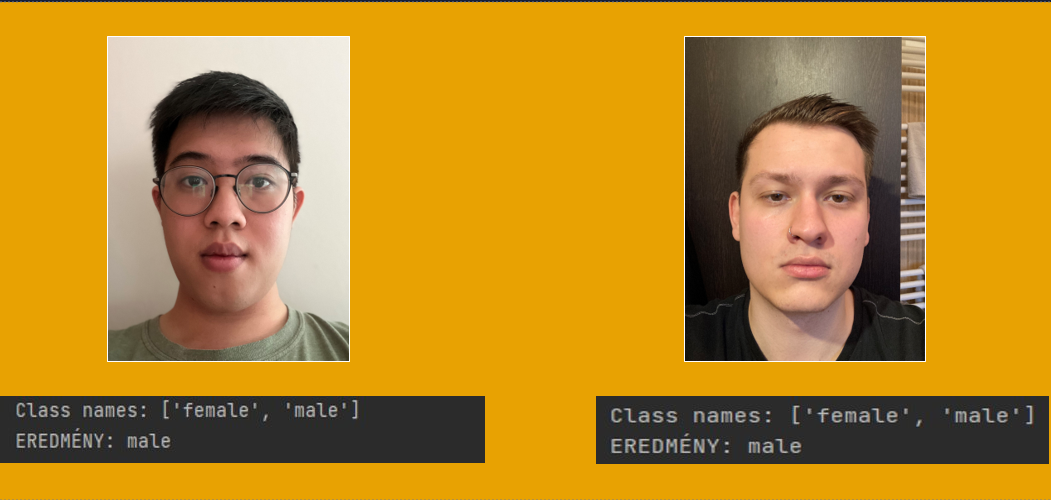
\includegraphics[width=1\linewidth]{gender}
        \caption{  A nemek klasszifikálására készült hálózat becslései.}
        \label{fig:gender}
	\end{figure}

    A(z) \ref{fig:gender}. ábrán láthatjuk a modellünk által becsült nemeket.

    \newpage
    \begin{figure}[h]	
		\centering
		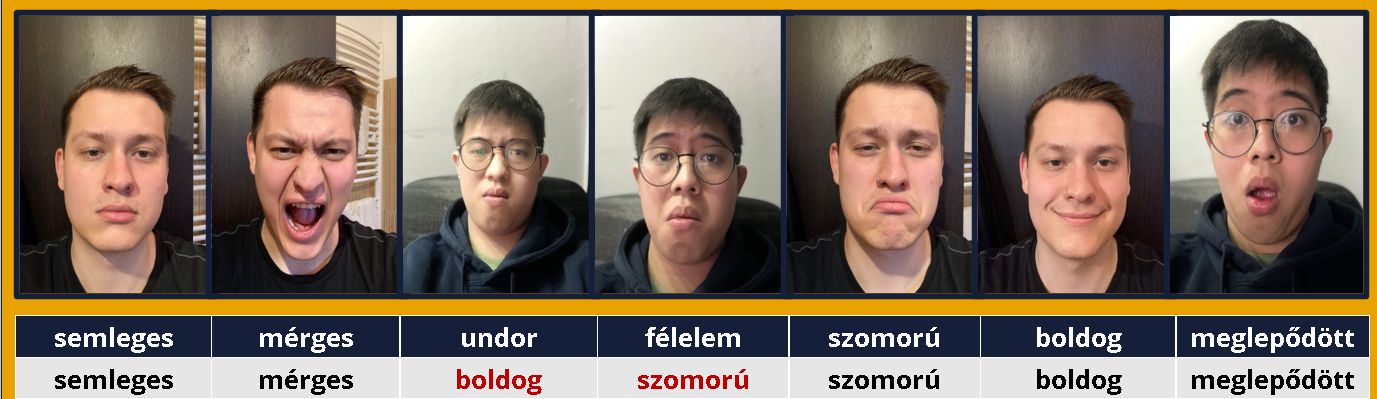
\includegraphics[width=1\linewidth]{arcanalizis}
        \caption{  Az arckifejezések klasszifikálására készült hálózat becslései.}
        \label{fig:expr}
	\end{figure}

    A(z) \ref{fig:expr}. ábrán 7 különböző arckifejezésre láthatjuk a becsléseket és megfigyelhetjük, hogy az undort és a félelmet a modellünk képtelen pontosan megbecsülni. Hogy pontosan lássuk a modell milyen kifejezésekre milyen pontossággal ad becslést, készitettünk egy konfuziós mátrixot, amely a(z) \ref{fig:cfmatrix}. ábrán látható.

    \begin{figure}[h!]	
		\centering
		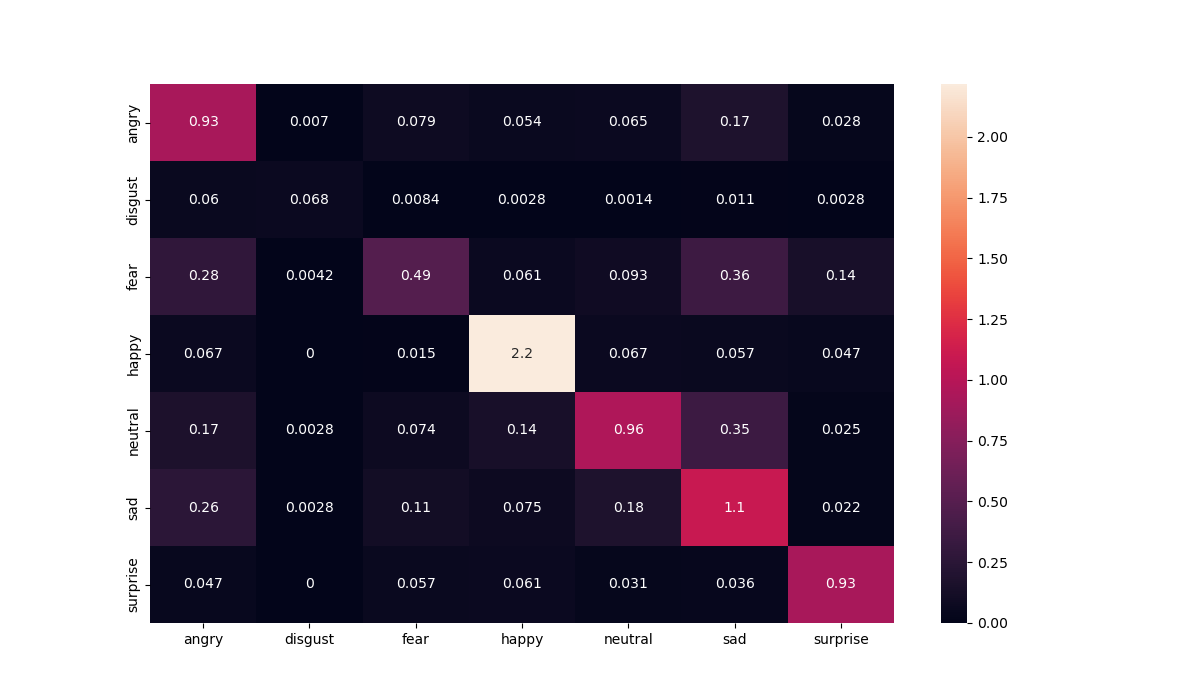
\includegraphics[width=1\linewidth]{output_cf_matrix.png}
        \caption{Az arckifejezések klasszifikálására készült hálózat konfuziós mátrixa.}
        \label{fig:cfmatrix}
	\end{figure}

    \subsubsection{Eredmények értékelése}
 
    \cite{facerecresult}Yoo és tsai. (2020) "Facial Expression Recognition Accuracy and Reaction Time Among Elementary School Students" című tanulmányának célja az volt, hogy megvizsgálja az általános iskolások pontosságát és reakcióidejét az arckifejezések felismerésében. A tanulmány szintén FER-2013 adathalmazt használta, amely 35 887 szürkeárnyalatos arcképből áll, amelyeket hét alapvető érzelem (harag, undor, félelem, boldogság, szomorúság, meglepetés és semleges) egyikével jelöltek meg.

    A tanulmányhoz 204 általános iskolás diákot vontak be, és arra kérték őket, hogy töltsenek ki egy arckifejezés-felismerési feladatot. A feladatban a tanulóknak egy sor arckifejezést mutattak, és arra kérték őket, hogy egy hét lehetőségből álló listából válasszák ki az arckifejezésnek leginkább megfelelő érzelmet. A vizsgálat során adatokat gyűjtöttek a diákok életkoráról, neméről és tanulmányi teljesítményéről is.

    A tanulmány megállapította, hogy az érzelmek felismerése a női modelleken jobbnak bizonyult, mint a
    a szomorúság esetében a férfi modellekhez képest (82,5\%-os és 72,0\%-os átlagos egyetértési arány),
    félelem (átlagos egyetértési arányok 75,2\% és 68,8\%), undor (átlagos egyetértési arányok
    84,2\% és 77,4\%) és a megvetés (átlagos egyetértési arány 77,5\% és 71,8\%). Az egyetértési arányok azonban magasabbak voltak a férfi, mint a női modellekben az alábbi esetekben
    harag (69,4\% és 60,6\%), meglepettség (96,1\% és 92,2\%),
    és a semleges arc (89,9\% és 86,9\%). 

    Általánosságban elmondható, hogy a bemutatott és a felismert érzelmek közötti átlagos százalékos egyezés
    82\% volt.

    
    
   \begin{figure}[h!]	
		\centering
		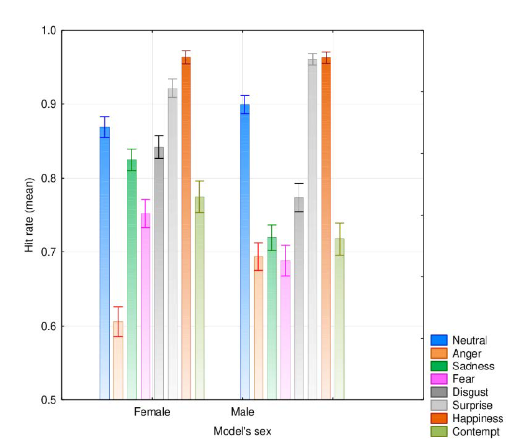
\includegraphics[width=1\linewidth]{facereqhuman.png}
        \caption{A különböző érzelmi kategóriák átlagos egyetértési aránya a modellek nemétől függően. Forrás: \cite{facerecresult}}
        \label{fig:humanfacerec}
	\end{figure}

    \begin{figure}[h!]	
		\centering
		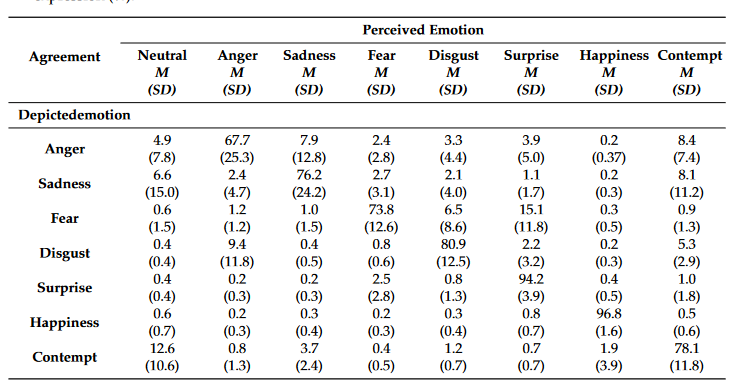
\includegraphics[width=1\linewidth]{facerechuman-confmatrix.png}
        \caption{A "találati arányok" átlaga és szórása (SD) arckifejezésenként (\%). Forrás: \cite{facerecresult}}
        \label{fig:humanfacerecmatrix}
	\end{figure}
    
    \subsection{Felhasználói felület}
	

	\newpage
	\renewcommand{\refname}{Hivatkozások}
	\begin{thebibliography}{9}
		
		\bibitem{tewari}
		Tewari, A., Zollhofer, M., Kim, H., Garrido, P., Bernard, F., Perez,
		P., Theobalt, C. (2017).
		\textit{Mofa: Model-based deep convolutional face au-
		toencoder for unsupervised monocular reconstruction. In Proceedings of
		the IEEE International Conference on Computer Vision Workshops (pp.
		1274-1283)}
		
		\bibitem{tran}
		Tuan Tran, A., Hassner, T., Masi, I., Medioni, G. (2017). 
		\textit{Regressing
		robust and discriminative 3D morphable models with a very deep neural
		network. In Proceedings of the IEEE conference on computer vision and
		pattern recognition (pp. 5163-5172)}
		
		\bibitem{olszewski}
		Olszewski, K., Lim, J. J., Saito, S., Li, H. (2016).
		\textit{High-fidelity facial and
		speech animation for VR HMDs. ACM Transactions on Graphics (TOG),
		35(6), 1-14}
		
		\bibitem{styner}
		Styner, M. A., Rajamani, K. T., Nolte, L. P., Zsemlye, G., Székely, G.,
		Taylor, C. J., Davies, R. H. (2003, July).
		\textit{ Evaluation of 3D correspondence
		methods for model building. In Biennial International Conference on In-
		formation Processing in Medical Imaging (pp. 63-75). Springer, Berlin,
		Heidelberg}
		
		\bibitem{survey} 
		Morales, A., Piella, G., Sukno, F. M. (2021). 
		\textit{Survey on 3D face re-
		construction from uncalibrated images. Computer Science Review, 40,
		100400.}
		
		\bibitem{auto}
		Kala, R. (2016).
		\textit{On-road intelligent vehicles: Motion planning for intel-
		ligent transportation systems. Butterworth-Heinemann.}	
		
		\bibitem{scanner}
		Kovacs, L., Zimmermann, A., Brockmann, G., Gühring, M., Baurecht,H., Papadopulos, N. A., ... Zeilhofer, H. F. (2006).
		\textit{Three-dimensional
		recording of the human face with a 3D laser scanner. Journal of plastic,
		reconstructive and aesthetic surgery, 59(11), 1193-1202}
		
		\bibitem{blanzvetter}
		Blanz, V., Vetter, T. (1999, July).
		\textit{A morphable model for the synthesis
		of 3D faces. In Proceedings of the 26th annual conference on Computer
		graphics and interactive techniques (pp. 187-194)}
		
		\bibitem{3dmm}
		Egger, B., Smith, W. A., Tewari, A., Wuhrer, S., Zollhoefer, M., Beeler,
		T.,... Vetter, T. (2020).
		\textit{3d morphable face models—past, present, and
		future. ACM Transactions on Graphics (TOG), 39(5), 1-38}
		
		\bibitem{dolphins}
		Cashman, T. J., Fitzgibbon, A. W. (2012).
		\textit{What shape are dolphins?
		building 3d morphable models from 2d images. IEEE transactions on pat-
		tern analysis and machine intelligence, 35(1), 232-244}
		
		\bibitem{photometric}
		Ackermann, J., Goesele, M. (2015).
		\textit{A survey of photometric stereo
			techniques. Foundations and Trends® in Computer Graphics and Vision,
			9(3-4), 149-254, 149–254.}
		
		\bibitem{multiplex}
		Hernández, C., Vogiatzis, G., Brostow, G. J., Stenger, B., Cipolla,
		R. (2007, October).
		\textit{Non-rigid photometric stereo with colored lights. In
			2007 IEEE 11th International Conference on Computer Vision (pp. 1-8).
			IEEE}
		
		\bibitem{hibrid}
		Nehab, D., Rusinkiewicz, S., Davis, J., Ramamoorthi, R. (2005).
		\textit{Efficiently combining positions and normals for precise 3D geometry. ACM transactions on graphics (TOG), 24(3), 536-543.}
			
		\bibitem{patelsmith}
		Patel, A., Smith, W. A. (2012).
		\textit{Driving 3D morphable models using shading cues. Pattern Recognition, 45(5), 1993-2004}
		
		\bibitem{ann}
		Abraham, A. (2005).
		\textit{Artificial neural networks. Handbook of measuring system design}
		
		\bibitem{ann2}
		Jain, A. K., Mao, J., Mohiuddin, K. M. (1996).
		\textit{Artificial neural networks: A tutorial. Computer, 29(3), 31-44}
		
		\bibitem{ann3}
		\textit{MARCELL, Borza. Mesterséges neurális hálózatok matematikai alapjai.}
		
		\bibitem{ann4}
		Tamás, K. (2002).
		\textit{A mesterséges neurális hálók a jövőkutatás
			szolgálatában.}
		
		\bibitem{krenker}
		Krenker, A., Bester, J., Kos, A. (2011).
		\textit{Introduction to the artificial neural networks. Artificial Neural Networks: Methodological Advances and
			Biomedical Applications. InTech, 1-18.}
		
		\bibitem{saragih}
		Saragih, J. M., Lucey, S., Cohn, J. F. (2011, March). 
		\textit{Real-time avatar
			animation from a single image. In 2011 IEEE International Conference
			on Automatic Face and Gesture Recognition (FG) (pp. 117-124). IEEE}
		
		\bibitem{CNN}
		Indolia, S., Goswami, A. K., Mishra, S. P., Asopa, P. (2018).
		\textit{ Conceptual
			understanding of convolutional neural network-a deep learning approach.
			Procedia computer science, 132, 679-688.}
	
	
	\bibitem{synthetic}
	Richardson, E., Sela, M., Kimmel, R. (2016, October). 
	\textit{3D face reconstruction by learning from synthetic data. In 2016 fourth international conference on 3D vision (3DV) (pp. 460-469). IEEE.}
	
	\bibitem{keras}
	Manaswi, N. K. (2018).
	\textit{Understanding and working with Keras. In Deep
		Learning with Applications Using Python (pp. 31-43). Apress, Berkeley,
		CA.}
	
	\bibitem{yudong}
	Guo, Y., Cai, J., Jiang, B., Zheng, J. (2018).
	\textit{Cnn-based real-time
		dense face reconstruction with inverse-rendered photo-realistic face images. IEEE transactions on pattern analysis and machine intelligence,
		41(6), 1294-1307.}
	
	\bibitem{elad}
	 Richardson, E., Sela, M., Kimmel, R. (2016, October).
	\textit{3D face reconstruction by learning from synthetic data. In 2016 fourth international conference on 3D vision (3DV) (pp. 460-469). IEEE.}
	
	\bibitem{yudeng}
	Deng, Y., Yang, J., Xu, S., Chen, D., Jia, Y., Tong, X. (2019).
	\textit{Accurate
		3d face reconstruction with weakly-supervised learning: From single image
		to image set. In Proceedings of the IEEE/CVF Conference on Computer
		Vision and Pattern Recognition Workshops (pp. 0-0)}
	
	\bibitem{chen}
	Chen, D., Hua, G., Wen, F., Sun, J. (2016, October). 
	\textit{Supervised transformer network for efficient face detection. In European Conference on
		Computer Vision (pp. 122-138). Springer, Cham.}
	
	\bibitem{kingma}
	Kingma, D. P., Ba, J. (2014).
	\textit{Adam: A method for stochastic optimization. arXiv preprint arXiv:1412.6980.}
	
	\bibitem{deca}
	Feng, Y., Feng, H., Black, M. J., Bolkart, T. (2021).
	\textit{Learning an animatable detailed 3D face model from in-the-wild images. ACM Transactions
		on Graphics (TOG), 40(4), 1-13.}
	
	\bibitem{focus}
	Li, C., Morel-Forster, A., Vetter, T., Egger, B., Kortylewski, A. (2021).
	\textit{To fit or not to fit: Model-based Face Reconstruction and Occlusion Segmentation from Weak Supervision. arXiv preprint arXiv:2106.09614.}
	
	\bibitem{flame}
	Tianye Li, Timo Bolkart, Michael. J. Black, Hao Li, and Javier Romero
	(2017).
	\textit{Learning a model of facial shape and expression from 4D scans.
		ACM Transactions on Graphics, (Proc. SIGGRAPH Asia) 36, 6 (2017),
		194:1–194:17.}
	
	\bibitem{liwen}
	Liwen Hu, Shunsuke Saito, Lingyu Wei, Koki Nagano, Jaewoo Seo, Jens
	Fursund, Iman Sadeghi, Carrie Sun, Yen-Chun Chen, and Hao Li. (2017).
	(2017).
	\textit{Avatar Digitization from a Single Image for Real-time Rendering. ACM
		Transactions on Graphics (TOG) 36, 6 (2017), 195:1–195:14.}
	
	\bibitem{bulat}
	Adrian Bulat and Georgios Tzimiropoulos (2017).
	\textit{How far are we from solving the 2D and 3D Face Alignment problem? (and a dataset of 230,000 3D facial landmarks). In International Conference on Computer Vision.}
	
	\bibitem{mohammed}
	Mohammed, S. B., Abdulazeez, A. M. (2021).
	\textit{Deep Convolution Neural
		Network for Facial Expression Recognition. PalArch’s Journal of Archaeology of Egypt/Egyptology, 18(4), 3578-3586.}
	
	\bibitem{arcface}
	Deng, J., Guo, J., Xue, N., and Zafeiriou, S. (2019).
	\textit{Arcface: Additive angular margin loss for deep face recognition. In Proceedings of the
		IEEE/CVF conference on computer vision and pattern recognition (pp.
		4690-4699).}
	
	\bibitem{feafa}
	Yan, Y., Lu, K., Xue, J., Gao, P., and Lyu, J. (2019, July).
	\textit{Feafa: A
		well-annotated dataset for facial expression analysis and 3d facial animation. In 2019 IEEE International Conference on Multimedia and Expo
		Workshops (ICMEW) (pp. 96-101). IEEE.}
	
	\bibitem{paysan}
	Paysan, P., Knothe, R., Amberg, B., Romdhani, S., and Vetter, T. (2009, September).
	\textit{A 3D face model for pose and illumination invariant
		face recognition. In 2009 sixth IEEE international conference on advanced
		video and signal based surveillance (pp. 296-301). Ieee.}

    \bibitem{PCA}
	Castelán, Mario, and Edwin R. Hancock.
	\textit{A simple coupled statistical model for 3d face shape recovery. 18th International Conference on Pattern Recognition (ICPR'06). Vol. 1. IEEE, 2006.}


    \bibitem{resnet}
	Kaiming He, Xiangyu Zhang, Shaoqing Ren, and Jian Sun.
	\textit{Deep Residual Learning for Image Recognition. In IEEE Conference on Computer Vision and Pattern Recognition  2016. (CVPR). 770–778.}

    \bibitem{tl}
    Weiss, Karl, Taghi M. Khoshgoftaar, and DingDing Wang.
    \textit{A survey of transfer learning." Journal of Big data 3.1 (2016): 1-40.}

    \bibitem{unet}
    Olaf Ronneberger, Philipp Fischer, and Thomas Brox.
    \textit{U-net: Convolutional networks for biomedical image segmentation. In International Conference on Medical image computing and computer-assisted intervention. Springer, 234–241 (2015.)}

    \bibitem{celeba}
    Liu, Z., Luo, P., Wang, X., Tang, X.
    \textit{Deep learning face attributes in the wild. In: Proceedings of the IEEE international conference on computer vision. 2015. p. 3730-3738.}

    \bibitem{ciresan}
    Ciresan, D.C., Gambardella, L.M., Giusti, A., Schmidhuber, J.
    \textit{Deep neural networks segment neuronal membranes in electron microscopy images. In: NIPS, pp. 2852–2860 (2012)}

    \bibitem{diffrenderer}
    Kato, Hiroharu, et al.
    \textit{Differentiable rendering: A survey. arXiv preprint arXiv:2006.12057 (2020).}

    \bibitem{facerecresult}
    Dores, Artemisa R., et al.
    \textit{Recognizing emotions through facial expressions: A largescale experimental study. International journal of environmental research and public health 17.20 (2020): 7420.}

	\end{thebibliography}

\end{document}